% ==============================================================================
% SAMSUNG INNOVATION CAMPUS - AI COURSE
% CAPSTONE PROJECT FINAL REPORT
% ==============================================================================
% Main Document File
% Compiler: XeLaTeX / LuaLaTeX
% Bibliography backend: Biber (IEEE style)
% ==============================================================================

\documentclass{sicaireport}

% Load Metadata Configuration
% ==============================================================================
% SIC-AI CAPSTONE PROJECT REPORT - METADATA CONFIGURATION
% ==============================================================================
% Fill in your team's project information below.
% This file centralizes all metadata so you do not need to edit it in multiple places.
% ==============================================================================

% Project Title
\newcommand{\projectTitle}{< Project Title >}

% Submission Date (Format: DD/MM/YY)
\newcommand{\projectDate}{< Date (DD/MM/YY) >}

% Course & Program Information (Default)
\newcommand{\courseName}{AI Course}
\newcommand{\programName}{Samsung Innovation Campus}
\newcommand{\reportType}{Capstone Project Final Report}

% Academic Administration Information (Fixed Defaults)
\newcommand{\className}{SIC-AI-N02}
\newcommand{\instructorName}{TS. Trần Quang Quý}

% Team Information
\newcommand{\teamName}{Team Name}

% Team Members
\newcommand{\memberOne}{<Member 1>}
\newcommand{\memberTwo}{<Member 2>}
\newcommand{\memberThree}{<Member 3>}
\newcommand{\memberFour}{<Member 4>}
\newcommand{\memberFive}{<Member 5>}

% Logo Path
\newcommand{\samsungLogoPath}{figures/samsung_logo.png}


% Load Additional Preamble & Package Settings
% ==============================================================================
% SIC-AI CAPSTONE PROJECT REPORT - PREAMBLE CONFIGURATION
% ==============================================================================
% This file contains additional package configurations, bibliography setup,
% hyperref settings, and document-wide utility commands.
% ==============================================================================

% IEEE Bibliography via BibLaTeX & Biber
\usepackage[
    backend=biber,
    style=ieee,
    sorting=none,
    doi=false,
    isbn=false,
    url=false
]{biblatex}
\addbibresource{references.bib}

% Hyperref Setup with Samsung Corporate Palette
\usepackage{hyperref}
\hypersetup{
    colorlinks=true,
    linkcolor=SamsungBlue,
    citecolor=SamsungBlue,
    filecolor=SamsungBlue,
    urlcolor=SamsungBlue,
    pdfauthor={\teamName},
    pdftitle={\projectTitle},
    pdfsubject={\reportType\ - \programName},
    pdfkeywords={Samsung Innovation Campus, AI Course, Capstone Project, Deep Learning, Artificial Intelligence}
}

% Additional Utility Macros
\newcommand{\code}[1]{\texttt{#1}}
\newcommand{\abbr}[2]{\textbf{#1} (#2)}

% Avoid the "Font shape LatinModernMono bold undefined" warning: keywords in colour only (no bold)
\lstset{keywordstyle=\color{SamsungBlue}}


\begin{document}

% ------------------------------------------------------------------------------
% 1. COVER PAGE & TITLE PAGE
% ------------------------------------------------------------------------------
\makecoverpage
\maketitledetailpage

% ------------------------------------------------------------------------------
% 2. FRONT MATTER
% ------------------------------------------------------------------------------
\pagenumbering{roman}
\setcounter{page}{1}

% Table of Contents
\renewcommand{\contentsname}{Content}
\tableofcontents
\clearpage

% List of Figures
\listoffigures
\clearpage

% List of Tables
\listoftables
\clearpage

% List of Abbreviations (Structural Template)
\chapter*{List of Abbreviations}
\addcontentsline{toc}{chapter}{List of Abbreviations}
\begin{table}[htbp]
    \renewcommand{\arraystretch}{1.4}
    \begin{tabularx}{\textwidth}{p{3.5cm} X}
        \toprule
        \textbf{Abbreviation} & \textbf{Full Definition / Description} \\
        \midrule
        \textbf{AI}           & Artificial Intelligence \\
        \textbf{SIC}          & Samsung Innovation Campus \\
        \textbf{EDA}          & Exploratory Data Analysis \\
        \textbf{ML}           & Machine Learning \\
        \textbf{DL}           & Deep Learning \\
        \textbf{CNN}          & Convolutional Neural Network \\
        \textbf{RNN}          & Recurrent Neural Network \\
        \textbf{NLP}          & Natural Language Processing \\
        \textbf{API}          & Application Programming Interface \\
        \textbf{UI}           & User Interface \\
        \bottomrule
    \end{tabularx}
\end{table}
\clearpage

% ------------------------------------------------------------------------------
% 3. MAIN MATTER
% ------------------------------------------------------------------------------
\pagenumbering{arabic}
\setcounter{page}{1}

\chapter{Introduction}
\label{chap:introduction}

\section{Background Information}
\label{sec:background}

% [TODO: Insert your project's background information here]
% Provide the domain context, problem area, and foundational technologies relevant to the project.

\section{Motivation and Objective}
\label{sec:motivation_objective}

% [TODO: Insert motivation and objective here]
% Describe the primary driving factors for this project and specific, measurable objectives.

\section{Members and Role Assignments}
\label{sec:members_roles}

% [TODO: Specify team members and detailed task/role assignments]

\begin{table}[htbp]
    \centering
    \caption{Team Members and Role Assignments}
    \label{tab:team_roles}
    \begin{tabularx}{\textwidth}{l p{3.8cm} X}
        \toprule
        \textbf{No.} & \textbf{Member Name} & \textbf{Assigned Roles and Responsibilities} \\
        \midrule
        1 & \memberOne   & Project Leader, System Architecture \\
        2 & \memberTwo   & Deep Learning Model Design and Training \\
        3 & \memberThree & Data Preprocessing and Feature Engineering \\
        4 & \memberFour  & Evaluation, Testing, and Optimization \\
        5 & \memberFive  & User Interface and Application Deployment \\
        \bottomrule
    \end{tabularx}
\end{table}

\section{Schedule and Milestones}
\label{sec:schedule_milestones}

% [TODO: Outline project schedule, timeline, and key milestones]

\begin{table}[htbp]
    \centering
    \caption{Project Timeline and Milestone Schedule}
    \label{tab:milestones}
    \begin{tabularx}{\textwidth}{c l X c}
        \toprule
        \textbf{Phase} & \textbf{Timeline} & \textbf{Key Deliverables / Activities} & \textbf{Status} \\
        \midrule
        1 & Weeks 1--2 & Topic selection, requirement analysis, and dataset acquisition & Completed \\
        2 & Weeks 3--4 & Exploratory Data Analysis (EDA) and data preprocessing & Completed \\
        3 & Weeks 5--7 & Model architecture design, baseline setup, and training & Completed \\
        4 & Weeks 8--9 & UI integration, testing, evaluation, and system optimization & In Progress \\
        5 & Week 10    & Final report submission and capstone presentation & Pending \\
        \bottomrule
    \end{tabularx}
\end{table}

\chapter{Project Execution}
\label{chap:project_execution}

\section{Data Acquisition}
\label{sec:data_acquisition}

% [TODO: Describe data sources, collection methods, dataset properties, and licensing]

\section{Training Methodology}
\label{sec:training_methodology}

% [TODO: Detail training methodology, hardware environment, loss functions, optimizers, and learning rate schedules]

\section{Workflow}
\label{sec:workflow}

% [TODO: Present the end-to-end pipeline workflow from raw input to inference output]

\section{System Design}
\label{sec:system_design}
% NOTE & TODO [SOURCE VARIATION NOTICE]:
% In the original Word template document (SIC_AI_Capstone Project_Final Report.docx):
% - Table of Contents (Page 3) uses: "2.4. System Diagram"
% - Chapter 2 Body Heading (Page 4) uses: "2.4. System Design"
% Following the project specification, the original section heading "System Design" is preserved here.
% If your instructor or committee prefers "System Diagram", you may adjust the heading text above.

\begin{figure}[htbp]
    \centering
    % Placeholder for system architecture diagram
    \setlength{\fboxrule}{0.8pt}%
    \setlength{\fboxsep}{20pt}%
    \fcolorbox{SamsungGray}{white}{%
        \parbox{0.85\textwidth}{%
            \centering\vspace{1.5cm}
            \sffamily\color{SamsungDarkGray}
            {\large\bfseries [System Architecture Diagram / Workflow Diagram]}\par
            \vspace{0.4cm}
            \footnotesize Replace this box with: \texttt{\textbackslash includegraphics[width=0.9\textbackslash textwidth]\{figures/system\_design.png\}}\par
            \vspace{1.5cm}
        }%
    }
    \caption{Overall System Architecture and Pipeline Flow}
    \label{fig:system_design}
\end{figure}

\chapter{Results}
\label{chap:results}

\section{Data Preprocessing}
\label{sec:data_preprocessing}

\subsection{Goals and Design Principles}
\label{subsec:prep_goals}

The preprocessing has two goals: to give every model a compact $224\times224$ input (the resolution of the pre-trained Vision Transformers), and to remove differences between the datasets that have nothing to do with the retina, such as the width of the black border. Three principles guided the design. First, \emph{one pipeline for all}: the same steps and the same constants are applied to every image of every dataset and every model. Second, \emph{no target information}: all constants were fixed before looking at DDR results, and no DDR statistic is used to adjust the preprocessing of EyePACS. Third, \emph{no hidden domain adaptation}: we deliberately do not apply colour normalisation such as Ben Graham's local-average subtraction, because it is itself a domain-normalisation method that would blur the effect we want to measure and would differ from the distribution on which RETFound was pre-trained.

\subsection{Pipeline}
\label{subsec:prep_pipeline}

For each image the following steps are performed (executed on Kaggle CPU kernels):

\begin{enumerate}[leftmargin=1.8em]
    \item \textbf{Label handling.} DDR images with the ``ungradable'' label are removed (346 images), leaving 3{,}759 test images.
    \item \textbf{Retina cropping.} The image is shrunk so that its longer side is 512 pixels, a pixel is considered background if all colour channels are $\le 15$ (out of 255), a row or column belongs to the retina if at least 1\% of its pixels are foreground, and the bounding box of those rows and columns, enlarged by a 2\% margin, is cropped from the full-resolution image. If no foreground is found, the whole image is kept (``fallback'').
    \item \textbf{Square padding.} The crop is padded with black to a square without distorting the aspect ratio, so that the optic disc and the macula keep their shape.
    \item \textbf{Resizing.} The square image is resized to $224\times224$ with Lanczos interpolation.
    \item \textbf{Cache.} The result is stored as a JPEG of quality 95 without chroma subsampling, so that all later experiments read small files instead of the original images (about 89\,GB for EyePACS).
    \item \textbf{Normalisation at load time.} Pixel values are scaled to $[0,1]$ and normalised with the ImageNet mean and standard deviation, as in the official RETFound fine-tuning code.
    \item \textbf{Duplicate check.} Near-duplicates between EyePACS and DDR would leak information from the source to the target domain, so every DDR test image is compared with all 88{,}702 EyePACS images. A coarse 64-bit difference hash (dHash) is computed first, followed by a stricter correlation test of a vessel-sensitive image descriptor (Section~\ref{subsec:prep_dup}).
\end{enumerate}

The cropping step matters because of the framing gap documented in Section~\ref{subsec:eda_domain_gap}: in DDR the retina occupies only about half of the image area, so without cropping the DDR retina would be much smaller than the EyePACS retina after resizing.

\subsection{Quality Checks and Preprocessing Result}
\label{subsec:prep_qa}

A packaging step verifies the cache: that every image listed in the manifest exists, that the image size is $224\times224$ (checked on a sample of about 300 images per split), and that no image failed to open; the number of images for which the cropping fell back to the whole image is also reported. All 92{,}461 images (35{,}126 + 10{,}906 + 42{,}670 EyePACS and 3{,}759 DDR) were processed in about 53 minutes on Kaggle CPU kernels, with \textbf{0 read errors, 0 missing cache files and 0 images with a wrong size} in the checked samples. The cropping fell back to the whole image for only \textbf{8 of the 92{,}461 images} (4 in EyePACS-train, 1 in EyePACS-validation, 3 in EyePACS-test, none in DDR), so the retina detector worked on 99.99\% of the images. The cache occupies 681.6\,MB (train), 211.8\,MB (validation), 829.5\,MB (EyePACS-test) and 79.1\,MB (DDR-test), against about 89\,GB of original EyePACS images.

Figure~\ref{fig:before_after} shows the effect on six EyePACS and six DDR images. In EyePACS the black border is already narrow, so the change is small, and the shape of the retina is preserved. In DDR the large black margins are removed and the retina fills the square, so that the optic disc, macula and vessels occupy a similar share of the input in both datasets. Elliptical DDR retinas stay elliptical, because the padding is applied after cropping and never stretches the image.

\begin{figure}[htbp]
    \centering
    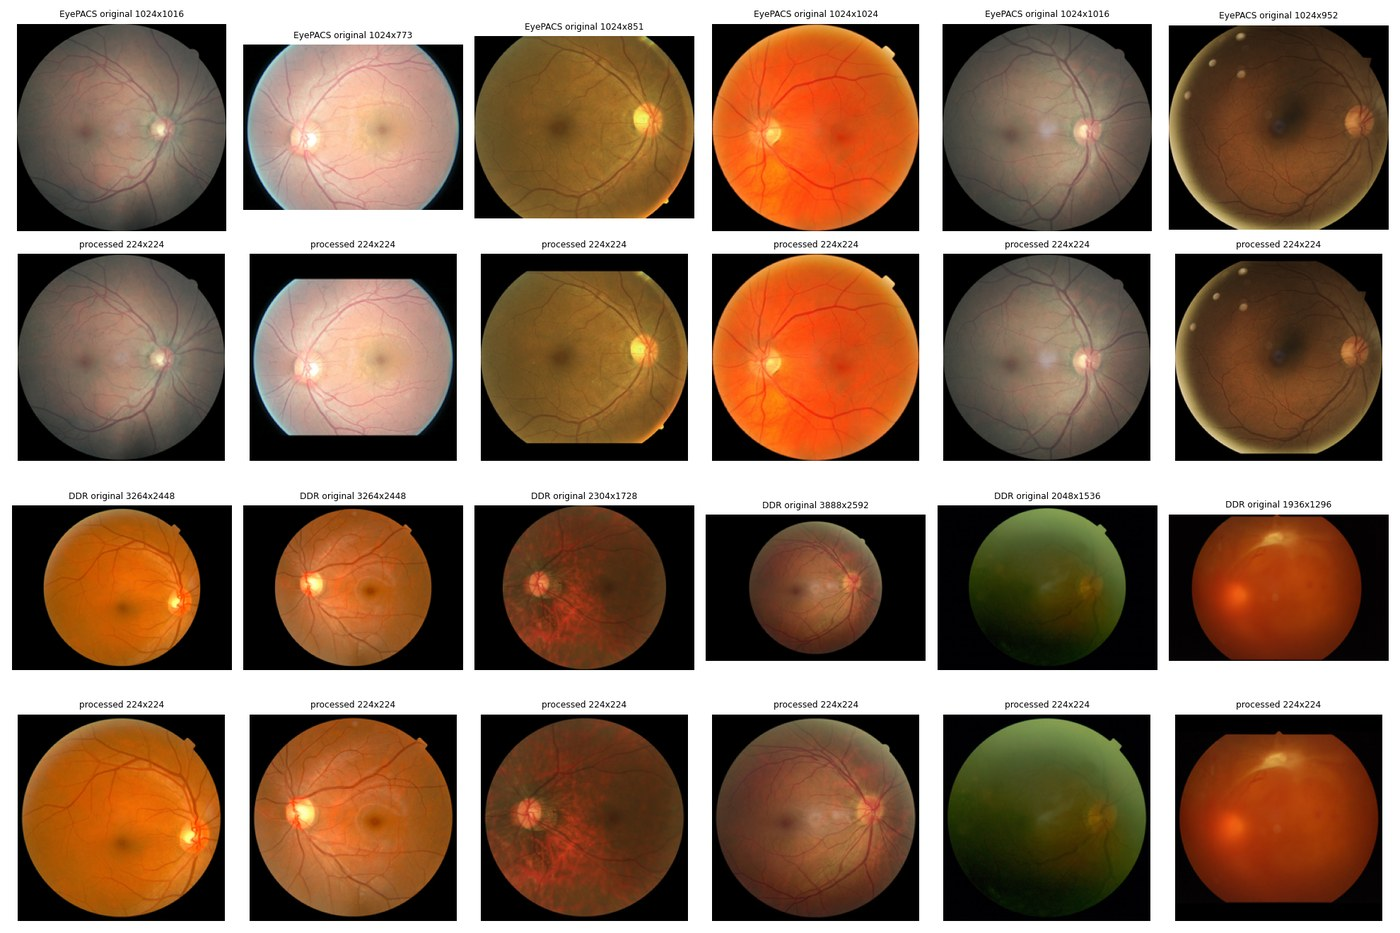
\includegraphics[width=0.9\textwidth]{figures/p01_before_after_crop.jpg}
    \caption{Preprocessing examples. For each dataset the first row shows the original image (with its size) and the second row the cropped, square-padded $224\times224$ result. Top two rows: EyePACS. Bottom two rows: DDR.}
    \label{fig:before_after}
\end{figure}

\subsection{Duplicate Check Between EyePACS and DDR}
\label{subsec:prep_dup}

The check has two stages, and the first one turned out to be too coarse. The 64-bit dHash (a $9\times8$ grayscale thumbnail) flagged 3{,}537 of the 3{,}759 DDR images (94\%) as being within 4 bits of some EyePACS image, 2{,}168 of them at distance 0. This does not mean that the datasets overlap: at this resolution all fundus photographs look alike, a bright disc on a black background, so the hash cannot tell different retinas apart. We therefore discarded the dHash as evidence and added a stricter test.

In the second stage each $224\times224$ image is converted to a $64\times64$ grayscale image, a Gaussian-blurred copy is subtracted so that mainly vessels and lesions remain, and the result is normalised to zero mean and unit length. Two images are compared by their normalised cross-correlation (NCC), which is 1 for identical content. To know which NCC values a true duplicate reaches, we ran a self-test: 300 randomly chosen DDR images were degraded (rescaled, JPEG quality 60, 15\% brighter), and each was compared with its original. The NCC of these copies was between 0.978 and 1.0 (median 0.995). The real DDR images, in contrast, reach a best NCC with any EyePACS image of only 0.80 on median, with a \textbf{maximum of 0.974}, which is below the \emph{lowest} value of the self-test copies (Figure~\ref{fig:dup_hist}). The six DDR images with the highest NCC were inspected visually (Figure~\ref{fig:dup_pairs}); in all six cases the most similar EyePACS image is a different retina that merely resembles the DDR image in framing and colour. We conclude that \textbf{no DDR test image has a near-duplicate in EyePACS} under re-compression, rescaling and brightness changes. The test is not designed to detect copies that were rotated, flipped or cropped; since the two datasets come from different countries and years and were released independently, we consider such copies unlikely, but this is a stated limitation.

\begin{figure}[htbp]
    \centering
    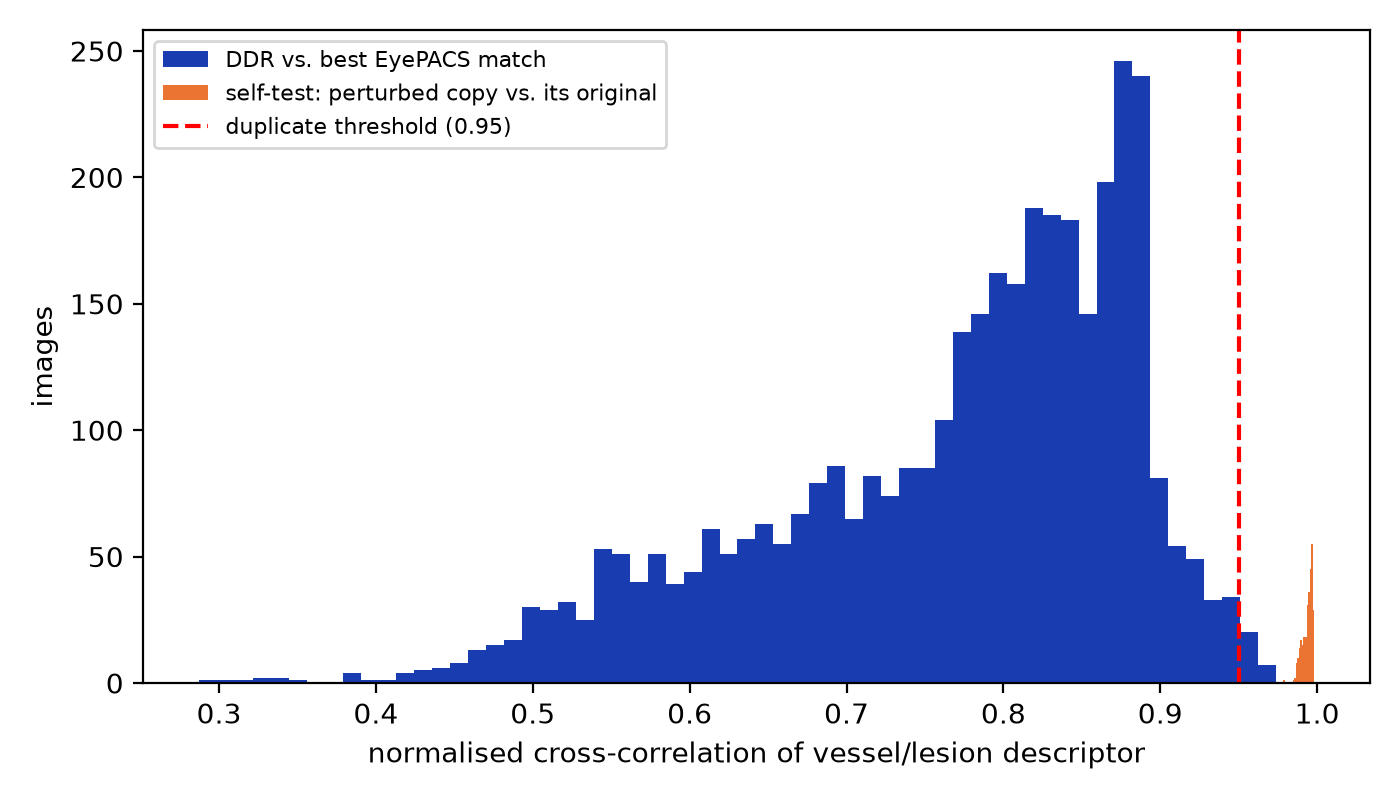
\includegraphics[width=0.78\textwidth]{figures/p03_dup_ncc_hist.png}
    \caption{Duplicate check. Blue: for each of the 3{,}759 DDR test images, the highest NCC with any EyePACS image. Orange: NCC between 300 artificially degraded DDR images and their originals (self-test). The two distributions do not overlap.}
    \label{fig:dup_hist}
\end{figure}

\begin{figure}[htbp]
    \centering
    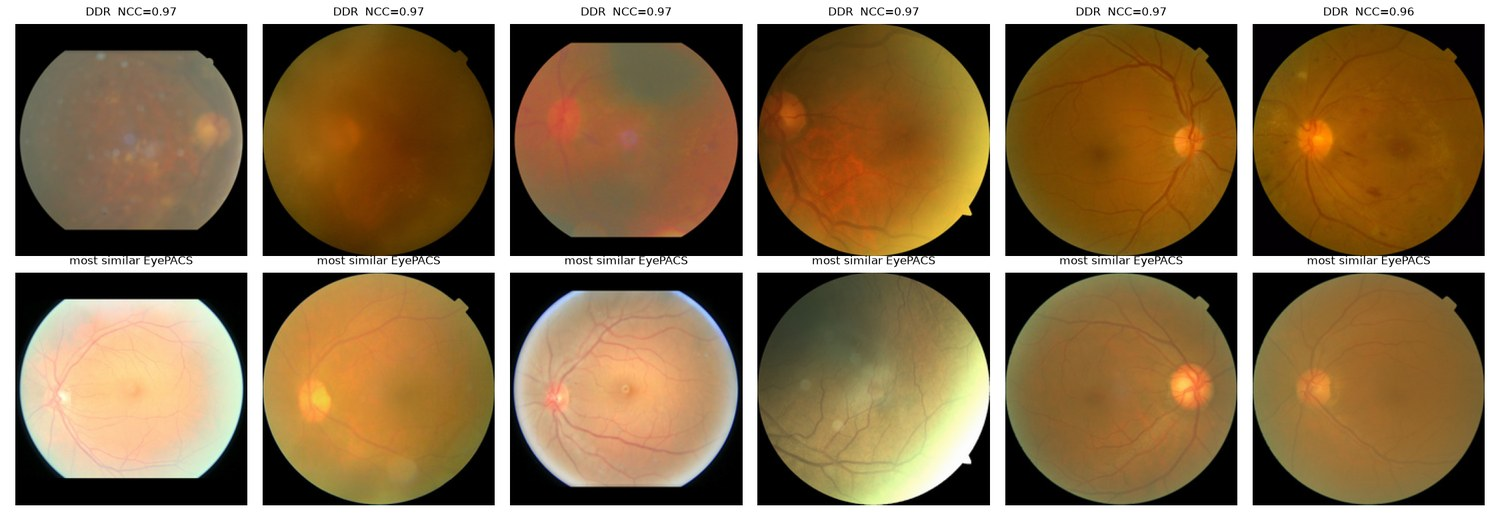
\includegraphics[width=0.92\textwidth]{figures/p04_dup_top_pairs.jpg}
    \caption{The six DDR images (top) with the highest correlation to an EyePACS image (bottom) are different retinas, not duplicates.}
    \label{fig:dup_pairs}
\end{figure}

\subsection{Augmentation During Training}
\label{subsec:prep_aug}

Augmentation is applied only to the training images, on the fly, after the cache is read. The augmentation is described in Section~\ref{subsec:augmentation}; the validation and test images only receive the normalisation of step~6.

\section{Exploratory Data Analysis (EDA)}
\label{sec:eda}

\subsection{Class Distributions and Label Shift}
\label{subsec:eda_labels}

Figure~\ref{fig:class_eyepacs} shows the grade distribution of the three EyePACS parts, and Figure~\ref{fig:class_ddr} that of DDR-test. The three EyePACS parts have almost the same proportions: grade~0 is 73.5\% of the training images, 74.5\% of the validation images and 73.6\% of the test images, whereas grade~3 and grade~4 together make up only about 4.5\%. In contrast, DDR-test has only 50.0\% of grade~0 but 35.8\% of grade~2 (EyePACS: about 15\%). The two datasets therefore differ in their label distribution, which is a \emph{label shift} on top of the covariate shift studied later. Two consequences follow: accuracy is not comparable across the datasets, and a model that has learned the EyePACS prior will tend to under-predict disease on DDR. Grade~3 is rare in both (71 images in DDR-test), so its recall will be uncertain.

\begin{figure}[htbp]
    \centering
    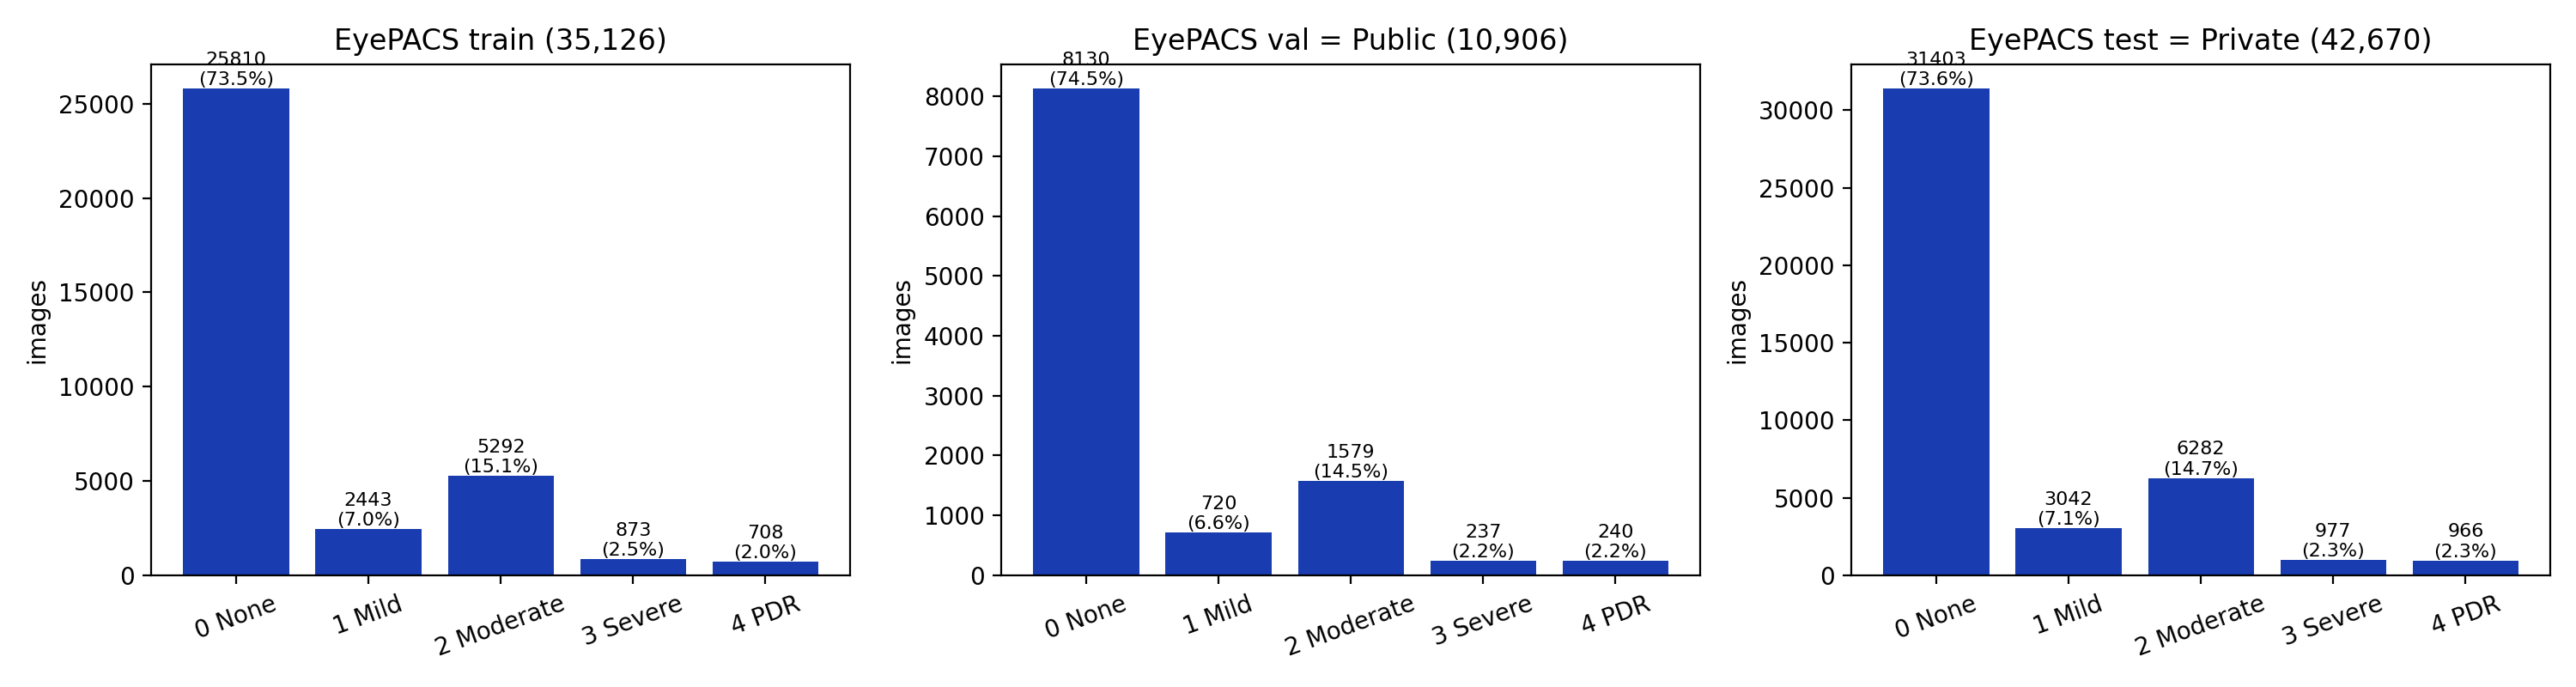
\includegraphics[width=\textwidth]{figures/d01_class_dist_eyepacs.png}
    \caption{Number of images per ICDR grade in the three EyePACS parts: training (left), validation = Public part of the test set (middle) and in-domain test = Private part (right). Percentages are shares of the part.}
    \label{fig:class_eyepacs}
\end{figure}

\begin{figure}[htbp]
    \centering
    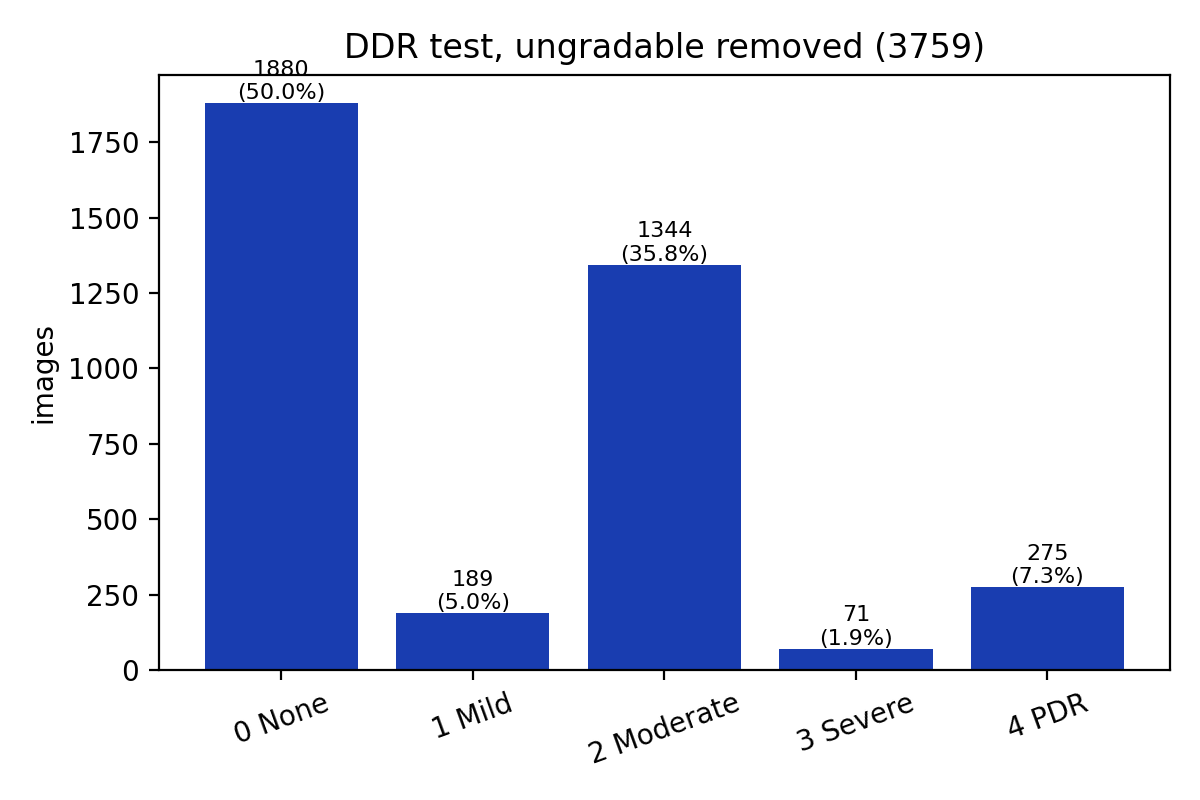
\includegraphics[width=0.62\textwidth]{figures/d02_class_dist_ddr.png}
    \caption{Number of images per ICDR grade in the DDR test split after removing ungradable images (3{,}759 images).}
    \label{fig:class_ddr}
\end{figure}

\subsection{Visual Comparison of the Two Domains}
\label{subsec:eda_samples}

Figure~\ref{fig:samples} shows randomly chosen images of every grade from EyePACS (top three rows) and from DDR (bottom three rows). Even for a human the origin is often recognisable: EyePACS images are mostly circular and fill the frame, with a variety of hues ranging from pale pink to red or dark green; DDR images are often elliptical with wide black margins and a more orange or yellow colour cast, and a few show strong green or very dark casts. Across both datasets, image quality varies widely, and some images of higher grades are blurred or partly obscured, which also explains part of the label noise of EyePACS.

\begin{figure}[htbp]
    \centering
    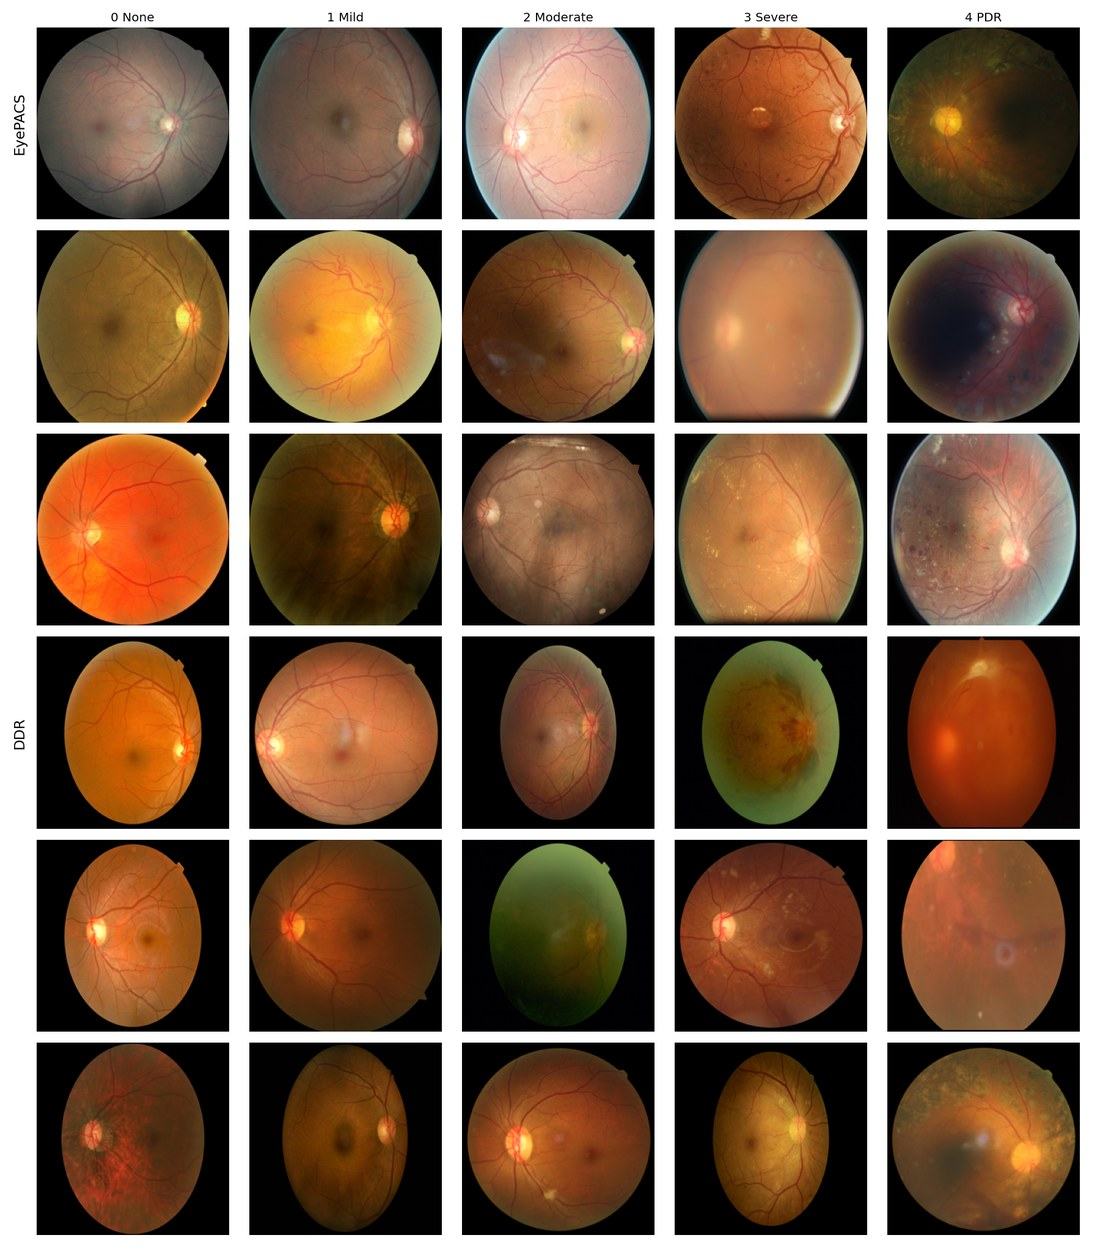
\includegraphics[width=0.92\textwidth]{figures/d03_samples_per_grade.jpg}
    \caption{Random samples per ICDR grade (columns 0--4). Top three rows: EyePACS. Bottom three rows: DDR. The two domains differ in framing (circular and tight vs. elliptical with black margins) and in colour.}
    \label{fig:samples}
\end{figure}

\subsection{Quantifying the Domain Gap}
\label{subsec:eda_domain_gap}

To quantify what the eye sees, we measured simple statistics on a random sample of 400 images from each dataset. The retina occupies about 83\% of the image area in the resized EyePACS images but only about 52\% in DDR, which confirms the need to crop. Figure~\ref{fig:color_stats} compares the mean intensity of each colour channel inside the retina. The red channel overlaps strongly, but the green and especially the blue channel of DDR are shifted towards lower values (blue: about 38 for DDR against about 67 for EyePACS), i.e.\ DDR images are on average warmer. This is a first, quantitative sign that the models will meet a colour shift at test time. Figure~\ref{fig:sizes} shows that the original resolutions also differ greatly: the resized EyePACS images have a longer side of at most 1{,}024 pixels (median about $1024\times946$), whereas DDR images are much larger (median about $2736\times1824$, up to $5184\times3456$). The orientation and exact shape of the retina vary as well.

\begin{figure}[htbp]
    \centering
    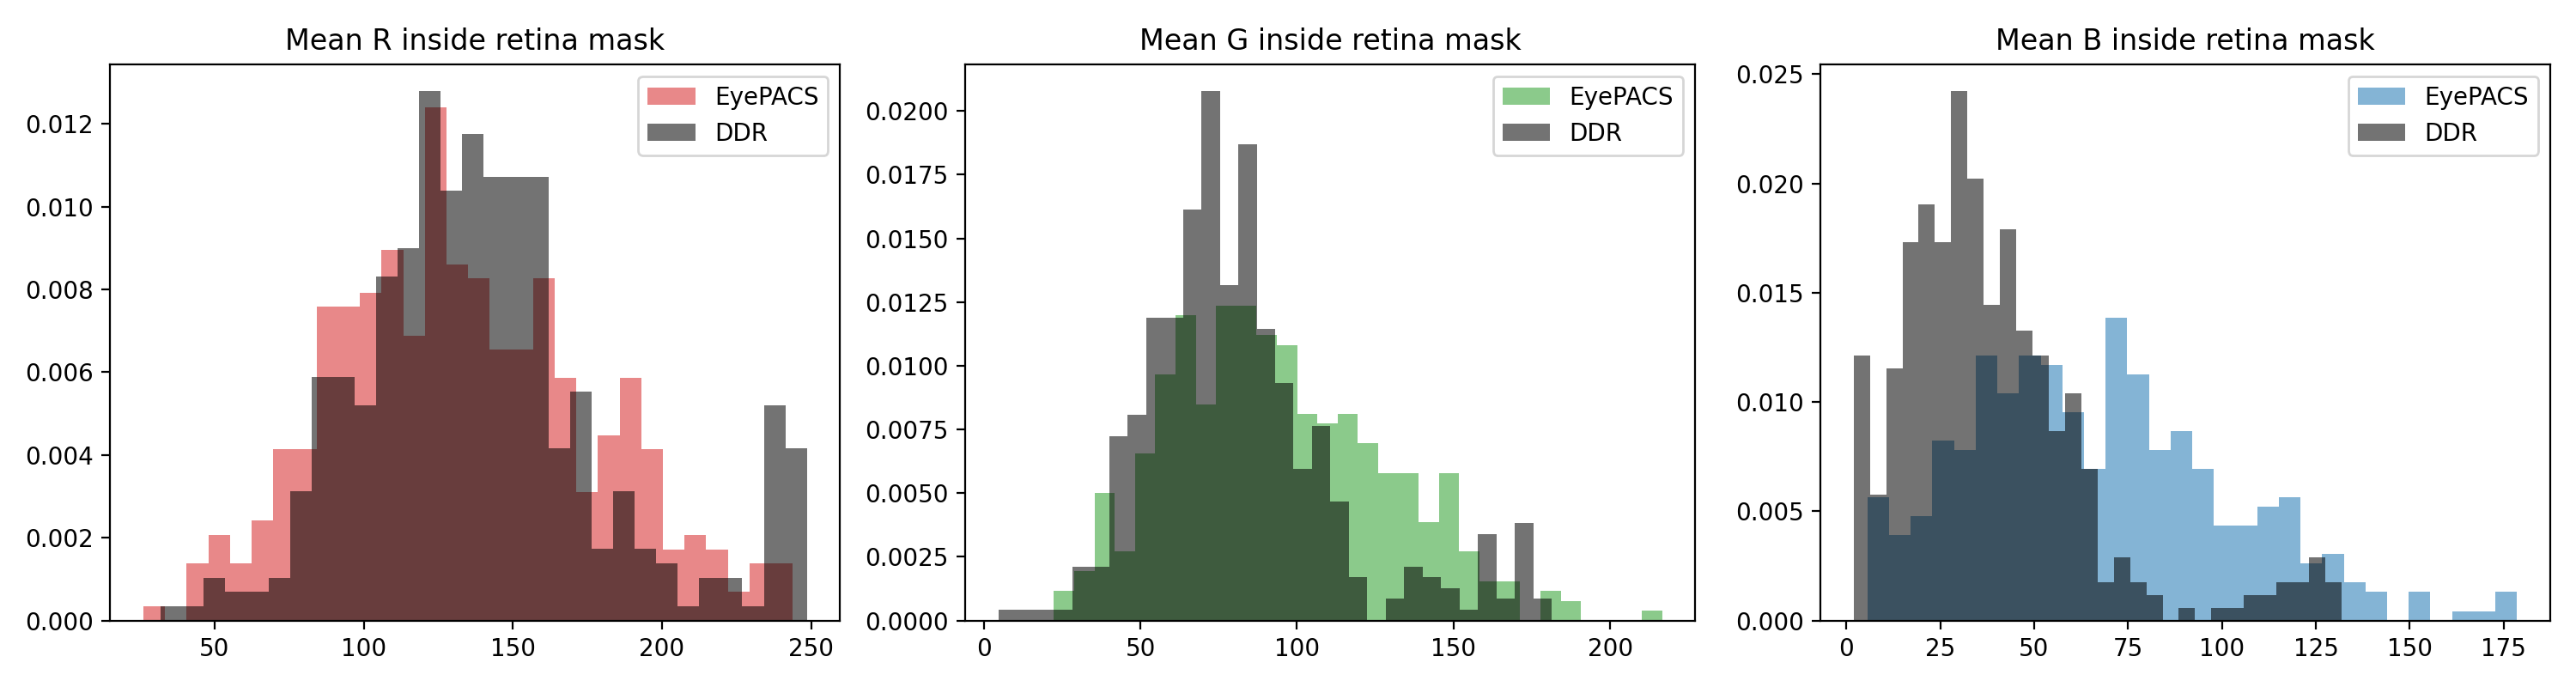
\includegraphics[width=0.92\textwidth]{figures/d04_color_stats_domain_gap.png}
    \caption{Histograms of the mean red, green and blue value inside the retina region for 400 random images per dataset. The blue (and, less strongly, green) channel of DDR is clearly shifted towards lower values.}
    \label{fig:color_stats}
\end{figure}

\begin{figure}[htbp]
    \centering
    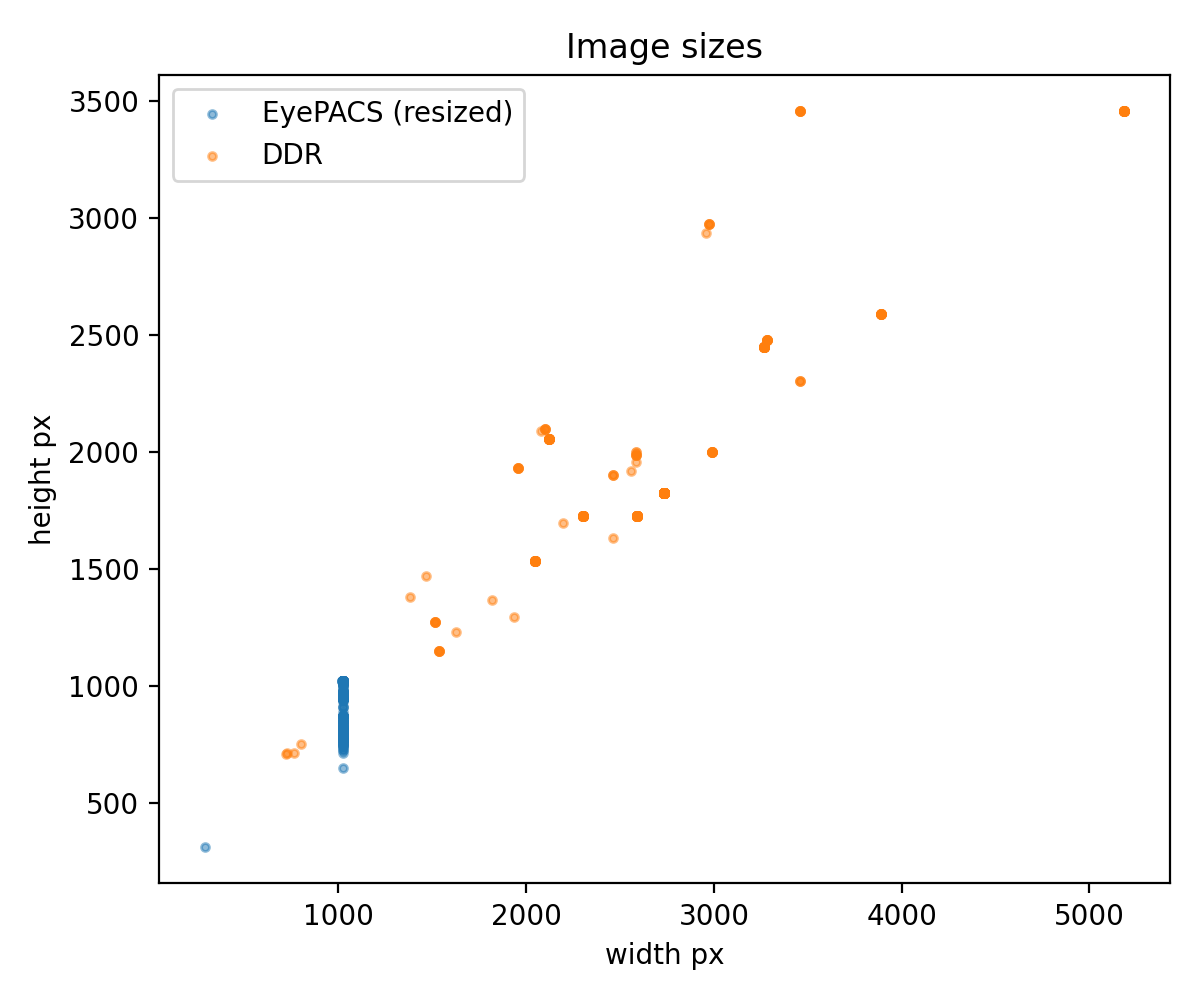
\includegraphics[width=0.62\textwidth]{figures/d05_image_sizes.png}
    \caption{Original image width and height of the sampled images. EyePACS (resized version) is concentrated at a width of about 1{,}024 pixels, while DDR images are larger and more varied.}
    \label{fig:sizes}
\end{figure}

\subsection{Findings Relevant to the Experiment}
\label{subsec:eda_findings}

The EDA leads to three concrete decisions and one observation:
\begin{itemize}[leftmargin=1.5em]
    \item Crop every image to the retina before resizing (framing gap).
    \item Use class-aware sampling and a robust loss (Section~\ref{subsec:loss}) because of the heavy imbalance of EyePACS.
    \item Report QWK, macro-F1 and per-grade recall instead of accuracy alone (label shift).
    \item \emph{Observation:} the colour gap suggests that colour augmentation could help; it was not applied in this study (Section~\ref{subsec:augmentation}), so the colour shift remains in the test conditions.
\end{itemize}

\section{Modeling}
\label{sec:modeling}

This section reports what the three models learned and how they behave on the two test sets. All numbers come from the saved predictions of the runs in Table~\ref{tab:experiments}; the tables are generated by script from these predictions, not typed by hand. The decision rule is the arg-max of the five class scores (the rule declared before training). Confidence intervals are 95\% paired bootstrap intervals over test images (1{,}000 resamples, shared across models) for the seed-0 runs.

\subsection{Training Dynamics}
\label{subsec:training_dynamics}

Figure~\ref{fig:curves} shows the EyePACS-validation QWK, macro-F1 and cross-entropy after each epoch. These are the only curves used to choose the checkpoint; the best epoch was epoch 5 for M1, epoch 11 for B2 and epoch 6 for both seeds of B1.

\begin{figure}[!htbp]
    \centering
    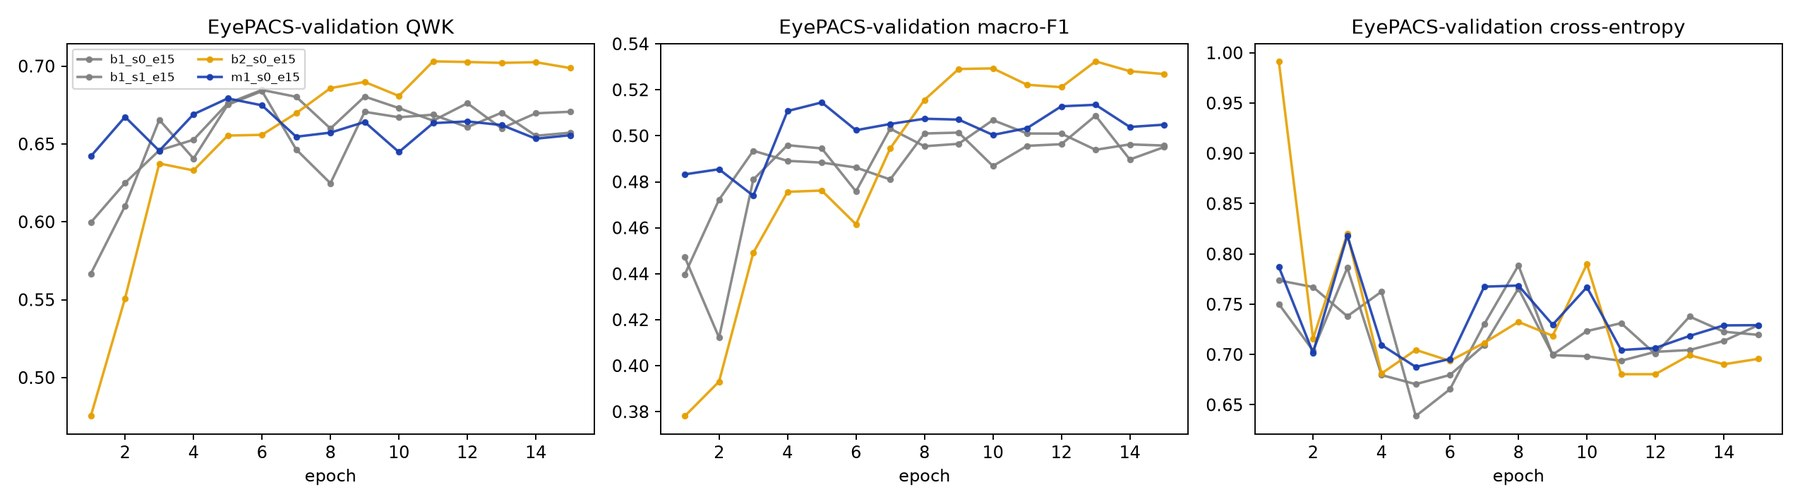
\includegraphics[width=\textwidth]{figures/t01_curves_all.jpg}
    \caption{EyePACS-validation QWK (left), macro-F1 (middle) and cross-entropy (right) per epoch for B1 (two seeds, grey), B2 (orange) and M1 (blue).}
    \label{fig:curves}
\end{figure}

The best validation QWK is 0.703 for B2, 0.685 and 0.684 for the two seeds of B1, and 0.679 for M1; at epoch~15 the values are 0.699, 0.671 and 0.657, and 0.656. B1 and M1 reach their plateau after five or six epochs. From then on the training loss keeps falling (M1: from 0.96 at epoch~5 to 0.65 at epoch~15) while the validation loss rises (M1: from 0.69 to 0.73) and the validation QWK does not improve, which is the usual sign of over-fitting. B2 learns more slowly and saturates at about 0.70 from epoch~11 (its last five values lie between 0.699 and 0.703). The two seeds of B1 have almost identical best values. Training for 15 epochs therefore did not raise the validation QWK beyond what was reached by epoch~11: under this recipe the number of epochs was not what limited the score. The final runs took 356~minutes (M1), 328~minutes (B2), and 50 and 48~minutes (B1, seeds 0 and 1).

\subsection{Main Results}
\label{subsec:main_results}

Table~\ref{tab:main_qwk} gives the primary metric. B1 is the mean and standard deviation of two seeds; its interval is that of seed~0.

\begin{table}[!htbp]
    \centering
    \caption{QWK on the in-domain test set (EyePACS-test, 42{,}670 images) and on the unseen target (DDR-test, 3{,}759 images). $\Delta$QWK is QWK(EyePACS-test) $-$ QWK(DDR-test); a negative value means that the score on DDR is \emph{higher}. Arg-max decision.}
    \label{tab:main_qwk}
    \footnotesize
    % Auto-generated by code/eval/analyze.py from results.json. Do not edit by hand.
\begin{tabularx}{\textwidth}{l c c c c}
\toprule
\textbf{Model} & \textbf{QWK (EyePACS-test)} & \textbf{QWK (DDR-test)} & \textbf{95\% CI (DDR, seed 0)} & $\boldsymbol{\Delta}$\textbf{QWK} \\
\midrule
B1 & 0.686 $\pm$ 0.002 & 0.701 $\pm$ 0.008 & [0.683, 0.726] & -0.015 $\pm$ 0.009 \\
B2 & 0.654 & 0.722 & [0.702, 0.741] & -0.068 \\
M1 & 0.680 & 0.691 & [0.668, 0.709] & -0.010 \\
M2 & 0.658 & 0.734 & [0.714, 0.753] & -0.076 \\
\bottomrule
\end{tabularx}
\end{table}

All three models lie close together. On EyePACS-test, B2 is first (0.686), followed by B1 (0.672) and M1 (0.670). On DDR-test the order is B2 (0.713), M1 (0.682) and B1 (0.669). The interval of B2 on DDR, [0.690, 0.734], overlaps slightly with those of M1 and B1; the paired comparison below, which uses the same resampled images for both models, is the sharper test.

\begin{table}[!htbp]
    \centering
    \caption{Secondary metrics on both test sets. Accuracy is reported for completeness; it is dominated by grade~0.}
    \label{tab:main_secondary}
    \footnotesize
    % Auto-generated
\begin{tabularx}{\textwidth}{l l c c c c}
\toprule
\textbf{Test set} & \textbf{Model} & \textbf{QWK} & \textbf{Macro-F1} & \textbf{AUC (referable)} & \textbf{Accuracy} \\
\midrule
EyePACS & B1 & 0.672 $\pm$ 0.003 & 0.477 $\pm$ 0.000 & 0.891 $\pm$ 0.003 & 0.782 $\pm$ 0.001 \\
EyePACS & B2 & 0.686 & 0.511 & 0.892 & 0.788 \\
EyePACS & M1 & 0.670 & 0.503 & 0.883 & 0.778 \\
\midrule
DDR & B1 & 0.669 $\pm$ 0.000 & 0.460 $\pm$ 0.015 & 0.893 $\pm$ 0.003 & 0.636 $\pm$ 0.040 \\
DDR & B2 & 0.713 & 0.503 & 0.893 & 0.682 \\
DDR & M1 & 0.682 & 0.461 & 0.874 & 0.596 \\
\bottomrule
\end{tabularx}
\end{table}

The AUC for referable DR is between 0.87 and 0.90 for every model and both datasets. B1 and B2 are practically identical (0.891--0.893), and M1 is slightly lower (0.883 in-domain, 0.874 on DDR). B2 also has the highest macro-F1 on both sets. The accuracy of B1 on DDR varies by 0.04 between its two seeds although its QWK does not, which shows how sensitive accuracy is to where the arg-max boundaries happen to fall.

\subsection{Why the In-Domain to Out-of-Domain Difference Needs Care}
\label{subsec:matched}

A negative $\Delta$QWK does not by itself mean that a model generalises better to DDR than to EyePACS. QWK depends on the grade mix of the test set: DDR has 50\% of grade~0 and 35.8\% of grade~2, whereas EyePACS has 73.6\% of grade~0 (Section~\ref{subsec:eda_labels}). DDR was also graded by a team of trained graders and its labels are probably cleaner than the single-grader EyePACS labels. To remove the first effect, the EyePACS-test images were resampled (stratified by grade) to the DDR grade mix before computing the QWK, and the bootstrap was repeated. Table~\ref{tab:matched} gives the result.

\begin{table}[!htbp]
    \centering
    \caption{Prior-matched comparison: QWK on EyePACS-test resampled to the DDR grade mix, QWK on DDR-test, and the matched $\Delta$QWK with 95\% bootstrap intervals (seed-0 runs).}
    \label{tab:matched}
    \small
    % Auto-generated
\begin{tabularx}{\textwidth}{l c c c}
\toprule
\textbf{Model} & \textbf{QWK EyePACS-test (DDR grade mix)} & \textbf{QWK DDR-test} & $\boldsymbol{\Delta}$\textbf{QWK (matched)} \\
\midrule
B1 & 0.671 [0.649, 0.693] & 0.670 [0.647, 0.694] & 0.002 [-0.030, 0.033] \\
B2 & 0.675 [0.655, 0.695] & 0.713 [0.690, 0.734] & -0.038 [-0.065, -0.010] \\
M1 & 0.676 [0.657, 0.695] & 0.682 [0.660, 0.702] & -0.006 [-0.033, 0.024] \\
\bottomrule
\end{tabularx}
\end{table}

After matching the grade mix, B1 ($\Delta=0.002$) and M1 ($\Delta=-0.006$) score the same on both datasets, and both intervals contain zero. B2 scores higher on DDR than on the matched EyePACS-test ($\Delta=-0.038$, interval [$-0.065$, $-0.010$]). None of the models therefore shows a measurable loss of QWK on the new domain. This should be read with care: the level on both datasets is only moderate, and the cleaner labels of DDR may hide part of a real domain effect.

\begin{figure}[!htbp]
    \centering
    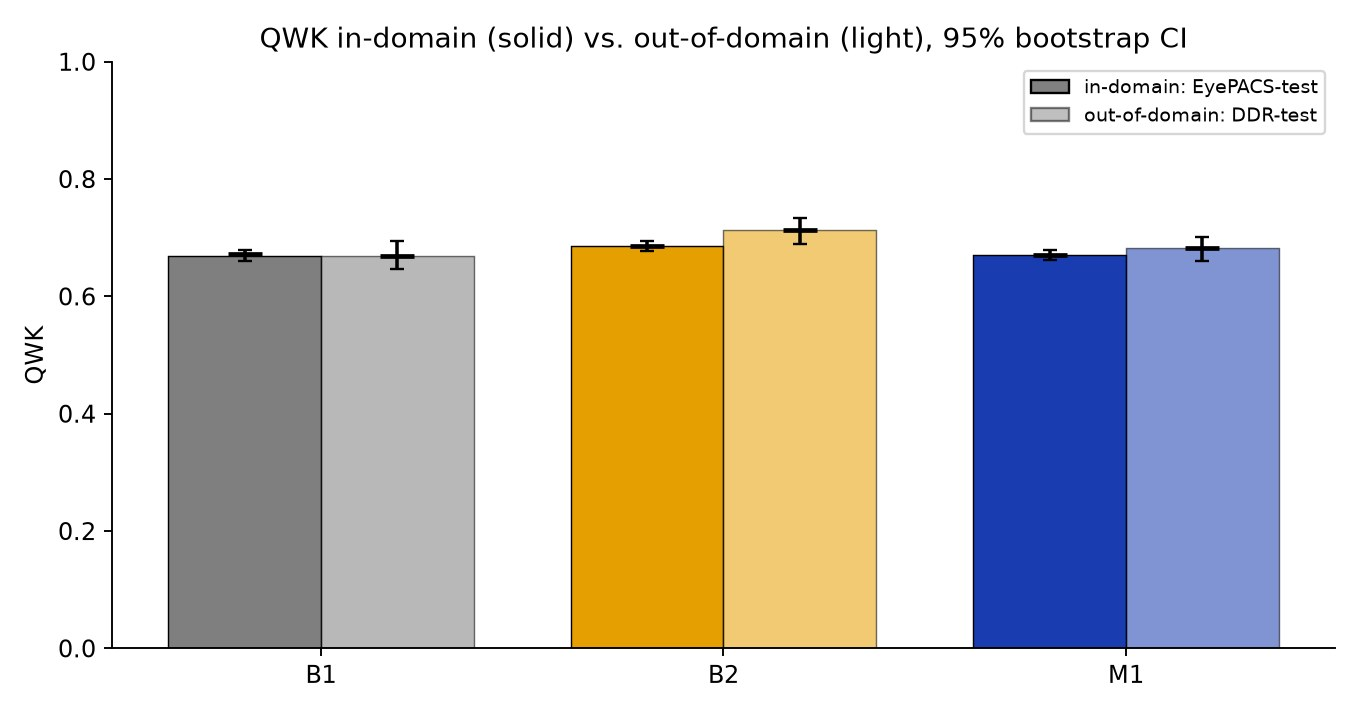
\includegraphics[width=0.7\textwidth]{figures/e04_inout.jpg}
    \caption{QWK in-domain (solid bars) and out-of-domain (light bars) with 95\% bootstrap intervals.}
    \label{fig:inout}
\end{figure}

\begin{figure}[!htbp]
    \centering
    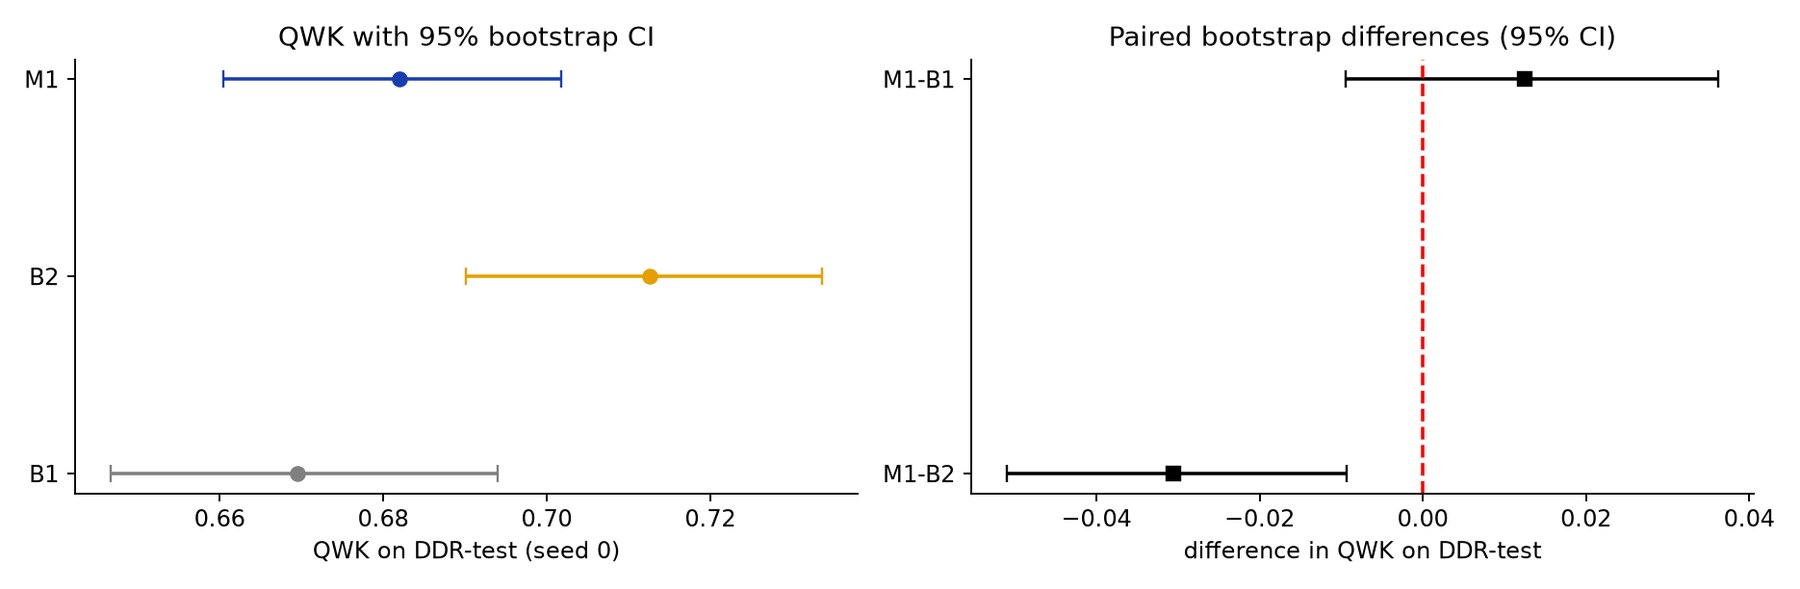
\includegraphics[width=0.9\textwidth]{figures/e05_bootstrap.jpg}
    \caption{Left: QWK on DDR-test with 95\% bootstrap intervals. Right: paired bootstrap differences of QWK on DDR-test; an interval that does not contain zero (red dashed line) indicates a difference larger than test-set sampling noise.}
    \label{fig:bootstrap}
\end{figure}

On DDR, the paired difference M1~$-$~B2 is $-0.031$ with a 95\% interval of [$-0.051$, $-0.009$]: M1 is \emph{worse} than B2 by more than test-sampling noise. The difference M1~$-$~B1 is $+0.013$ [$-0.009$, $0.036$] and cannot be distinguished from zero. For the in-to-out difference $\Delta$QWK, the raw contrasts are not distinguishable from zero (M1~$-$~B2: $0.015$ [$-0.007$, $0.037$]; M1~$-$~B1: $-0.012$ [$-0.037$, $0.013$]). On the prior-matched set, M1~$-$~B2 is $0.031$ [$0.005$, $0.060$], so B2 is also favoured in the matched in-to-out comparison, and M1~$-$~B1 remains undecided ($-0.008$ [$-0.041$, $0.023$]). All these intervals measure the sampling noise of the test images only, not the variation between training runs.

\subsection{Per-Grade Behaviour}
\label{subsec:per_grade}

Figure~\ref{fig:confusion} shows row-normalised confusion matrices (each row is a reference grade) for every model on both test sets, and Table~\ref{tab:recall} the recall per grade on DDR.

\begin{figure}[!htbp]
    \centering
    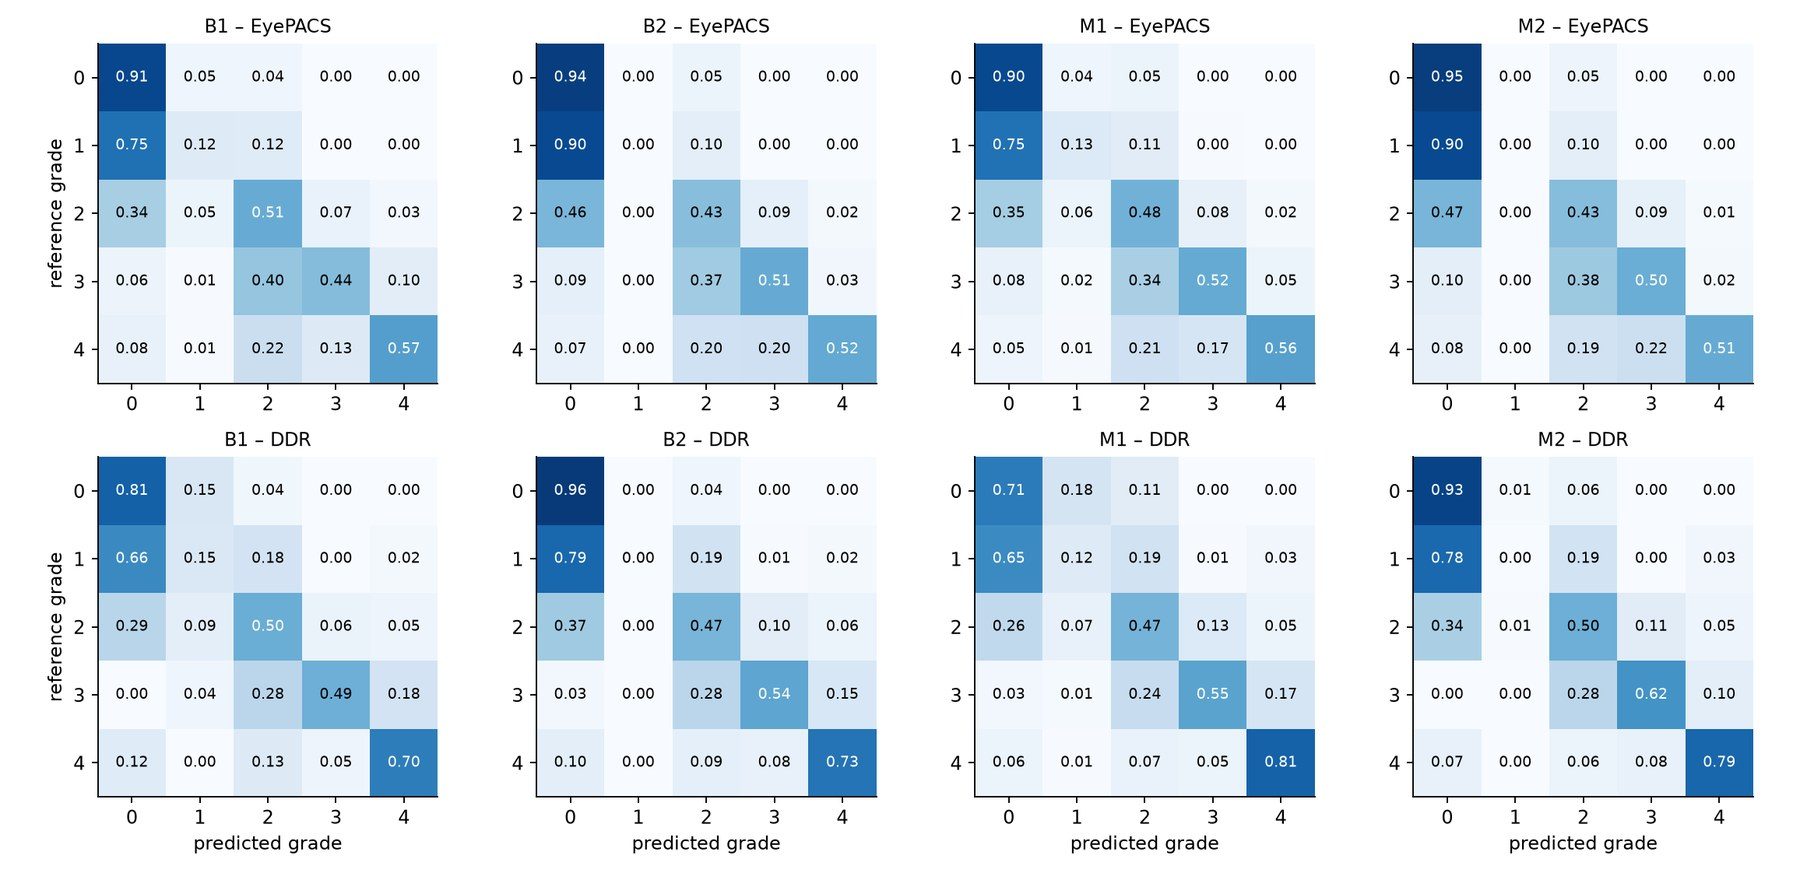
\includegraphics[width=0.92\textwidth]{figures/e01_confusion.jpg}
    \caption{Row-normalised confusion matrices of the seed-0 runs on EyePACS-test (top) and DDR-test (bottom). Rows: reference grade; columns: predicted grade.}
    \label{fig:confusion}
\end{figure}

\begin{table}[!htbp]
    \centering
    \caption{Recall per ICDR grade on DDR-test.}
    \label{tab:recall}
    \small
    % Auto-generated
\begin{tabularx}{\textwidth}{l c c c c c}
\toprule
\textbf{Model (DDR-test)} & \textbf{Grade 0} & \textbf{Grade 1} & \textbf{Grade 2} & \textbf{Grade 3} & \textbf{Grade 4} \\
\midrule
B1 & 0.802 & 0.152 & 0.519 & 0.474 & 0.679 \\
B2 & 0.958 & 0.000 & 0.466 & 0.535 & 0.735 \\
M1 & 0.710 & 0.122 & 0.475 & 0.549 & 0.807 \\
M2 & 0.926 & 0.000 & 0.496 & 0.620 & 0.789 \\
\bottomrule
\end{tabularx}
\end{table}

Grade~0 is recognised best (recall 0.77--0.86). Grade~1 is almost never recognised (0.06--0.11): most mild cases are predicted as no DR. Grade~2 recall is only 0.40--0.53; about a third of these images are predicted as grade~0 by the seed-0 runs and a further part as grade~3 or~4. M1 has the highest recall for grades~3 and~4 (0.66 and 0.74) and the lowest for grades~0 and~2, that is, it grades more aggressively. The B1 values are means of two seeds, and the seeds differ strongly although their QWK is the same: the recall of grade~3 is 0.20 for seed~0 and 0.73 for seed~1, and that of grade~2 is 0.56 and 0.34. Per-grade differences between the single-seed models B2 and M1 should therefore not be over-interpreted, especially for grade~3 with its 71 images.

\subsection{Referable Diabetic Retinopathy}
\label{subsec:referable}

For screening, the practically important question is whether an eye needs referral (grade $\geq 2$). Figure~\ref{fig:roc} shows the ROC curves on both test sets, computed from the total probability of grades 2--4.

\begin{figure}[!htbp]
    \centering
    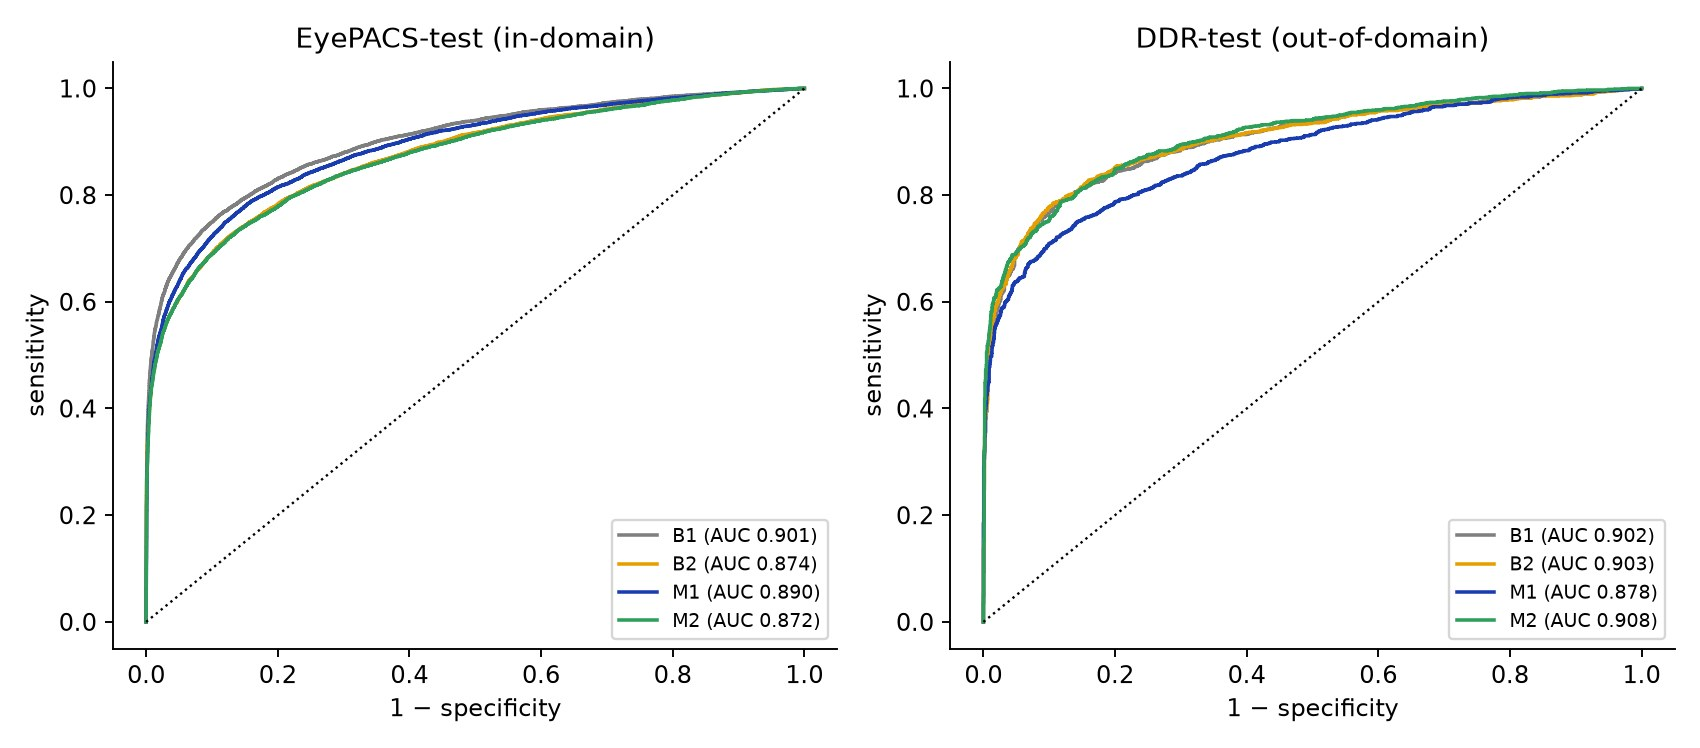
\includegraphics[width=0.85\textwidth]{figures/e02_roc.jpg}
    \caption{ROC curves of the seed-0 runs for referable DR (grade $\geq 2$) on EyePACS-test (left) and DDR-test (right).}
    \label{fig:roc}
\end{figure}

The curves of the three models are close to each other in-domain; on DDR, B2 lies above the others at low false-positive rates and M1 lies lowest over much of the middle range. The AUC on DDR (B1 0.893, B2 0.893, M1 0.874) is about the same as in-domain, so the ability to rank referable above non-referable eyes transfers to DDR. The ranking quality is better than the fixed arg-max operating point suggests: with the arg-max rule the referable sensitivity of the seed-0 runs on DDR is only 67--71\% at a specificity of 91--94\% (Table~\ref{tab:errors}). A screening deployment would need a lower, explicitly chosen threshold, fitted on validation data.

\subsection{Effect of the Decision Rule}
\label{subsec:decision_rule}

The arg-max rule ignores the ordering of the grades. As a secondary analysis, the five probabilities were converted into an expected grade, and four thresholds on it were fitted on \emph{EyePACS-validation only} to maximise QWK; no DDR image was used. Table~\ref{tab:ordinal} shows the result.

\begin{table}[!htbp]
    \centering
    \caption{QWK with ordinal decoding (expected grade and thresholds fitted on EyePACS-validation). B1 is the mean over two seeds.}
    \label{tab:ordinal}
    \footnotesize
    % Auto-generated by ordinal_variant.py
\begin{tabularx}{\textwidth}{l c c c c}
\toprule
\textbf{Model} & \textbf{QWK val (fit)} & \textbf{QWK EyePACS-test} & \textbf{QWK DDR-test} & \textbf{95\% CI (DDR, seed 0)} \\
\midrule
B1 & 0.725 $\pm$ 0.005 & 0.714 $\pm$ 0.004 & 0.709 $\pm$ 0.008 & [0.698, 0.735] \\
B2 & 0.740 & 0.721 & 0.734 & [0.714, 0.753] \\
M1 & 0.715 & 0.708 & 0.707 & [0.687, 0.725] \\
\bottomrule
\end{tabularx}
\end{table}

Ordinal decoding raises the QWK of every model: on DDR from 0.669 to 0.709 for B1, from 0.713 to 0.734 for B2 and from 0.682 to 0.707 for M1, with similar or larger gains in-domain. B2 remains first and M1 and B1 remain essentially tied. The best result of the study is thus a QWK of 0.734 on DDR (B2, ordinal decoding). This is well short of the level of 0.85 that the team had hoped to reach. Likely contributors are the small input size of $224\times224$ pixels, the noisy single-grader training labels and a loss function that ignores the order of the grades; the experiments of this study did not isolate the effect of any of them, and more epochs alone did not help (Section~\ref{subsec:training_dynamics}).

\subsection{Interpretability}
\label{subsec:interpretability}

Grad-CAM was computed for the last transformer block of M1 and B2 on DDR images: three images that M1 classified correctly and three that it classified wrongly, with the same images shown for both models (Figure~\ref{fig:gradcam}).

\begin{figure}[!htbp]
    \centering
    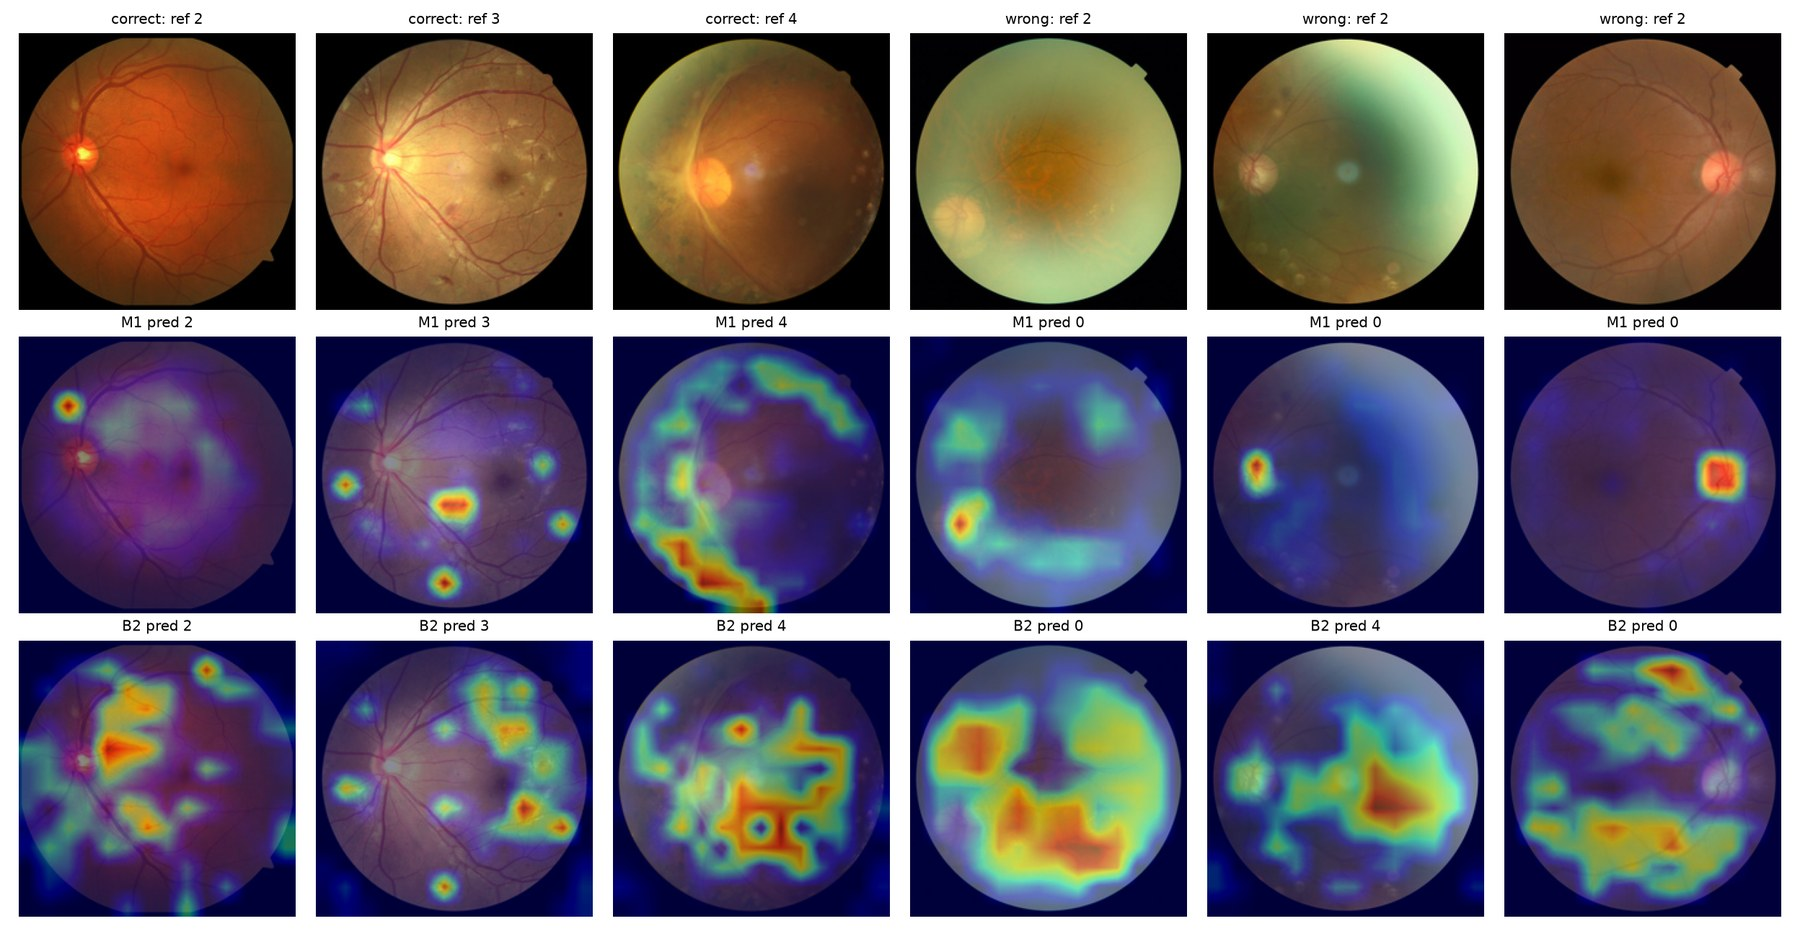
\includegraphics[width=0.92\textwidth]{figures/a01_gradcam.jpg}
    \caption{Grad-CAM on DDR-test images. Top: image with reference grade; middle: M1 heat map and prediction; bottom: B2 heat map and prediction. The first three columns are correct cases of M1, the last three are wrong cases.}
    \label{fig:gradcam}
\end{figure}

The images were drawn at random with a fixed seed: one correct M1 prediction for each of the grades 2, 3 and~4, and three images on which M1 was wrong by two or more grades. In the correct cases of Figure~\ref{fig:gradcam}, M1 puts its strongest response on a few compact spots (grade~2 and~3) and along the periphery and rim of the retina (grade~4); in the grade-3 image some of the spots lie near visible dark lesions, others do not. The maps of B2 are broader and in places reach outside the retina. In the three wrong cases the reference is grade~2 and M1 predicts grade~0; the first two photographs are visibly degraded (haze, a strong illumination gradient) and the third is dim. There the strongest M1 response is on the optic disc or near the rim, not on lesions, and the B2 maps are diffuse. These six images are a qualitative illustration and cannot show how often either behaviour occurs; Grad-CAM on a $14\times14$ patch grid is also coarse compared with the size of the smallest lesions.

Figure~\ref{fig:tsne_domain} shows a t-SNE embedding of the encoder features of 1{,}500 random test images of each dataset, coloured by dataset, and Figure~\ref{fig:tsne_grade} the same embedding coloured by grade.

\begin{figure}[!htbp]
    \centering
    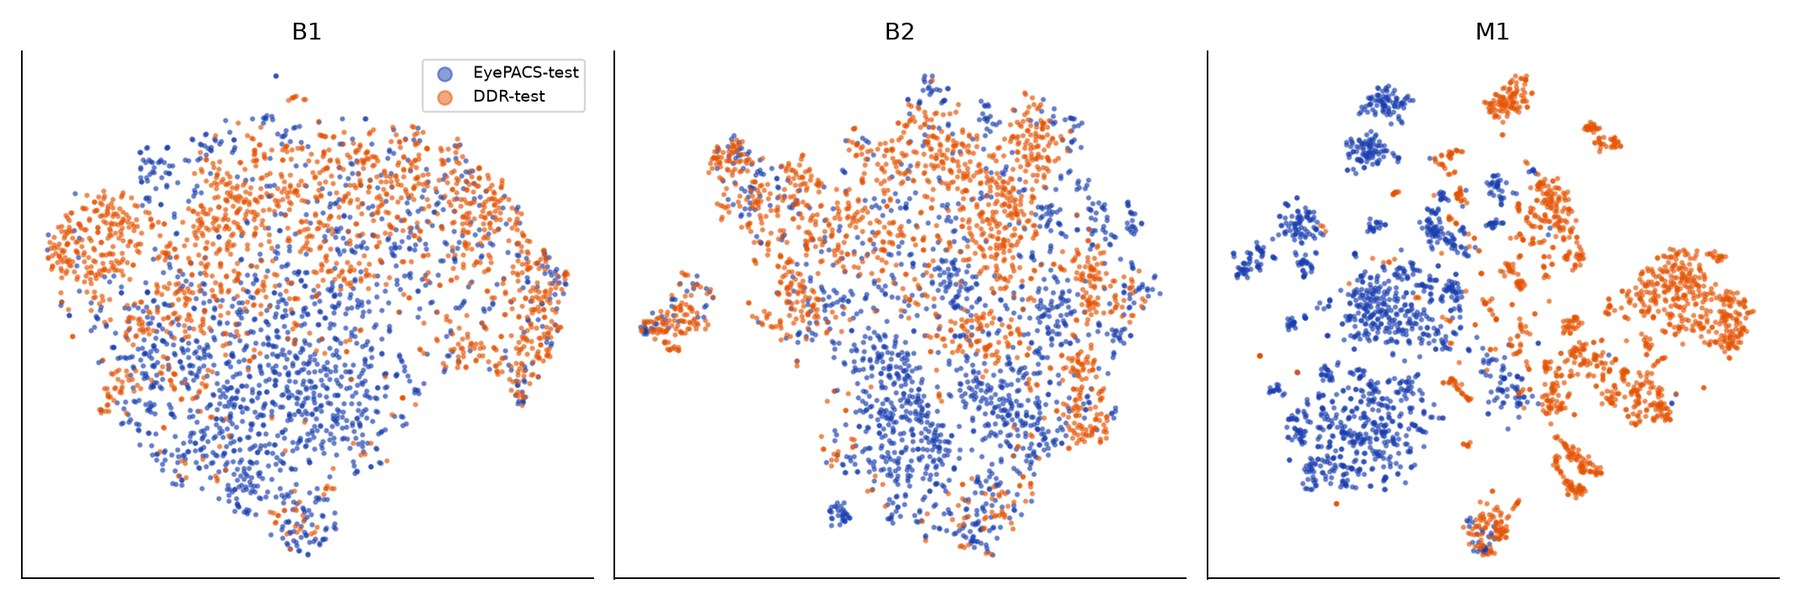
\includegraphics[width=0.9\textwidth]{figures/a03_tsne_domain.jpg}
    \caption{t-SNE of the encoder features coloured by dataset (blue: EyePACS-test, orange: DDR-test) for B1, B2 and M1.}
    \label{fig:tsne_domain}
\end{figure}

\begin{figure}[!htbp]
    \centering
    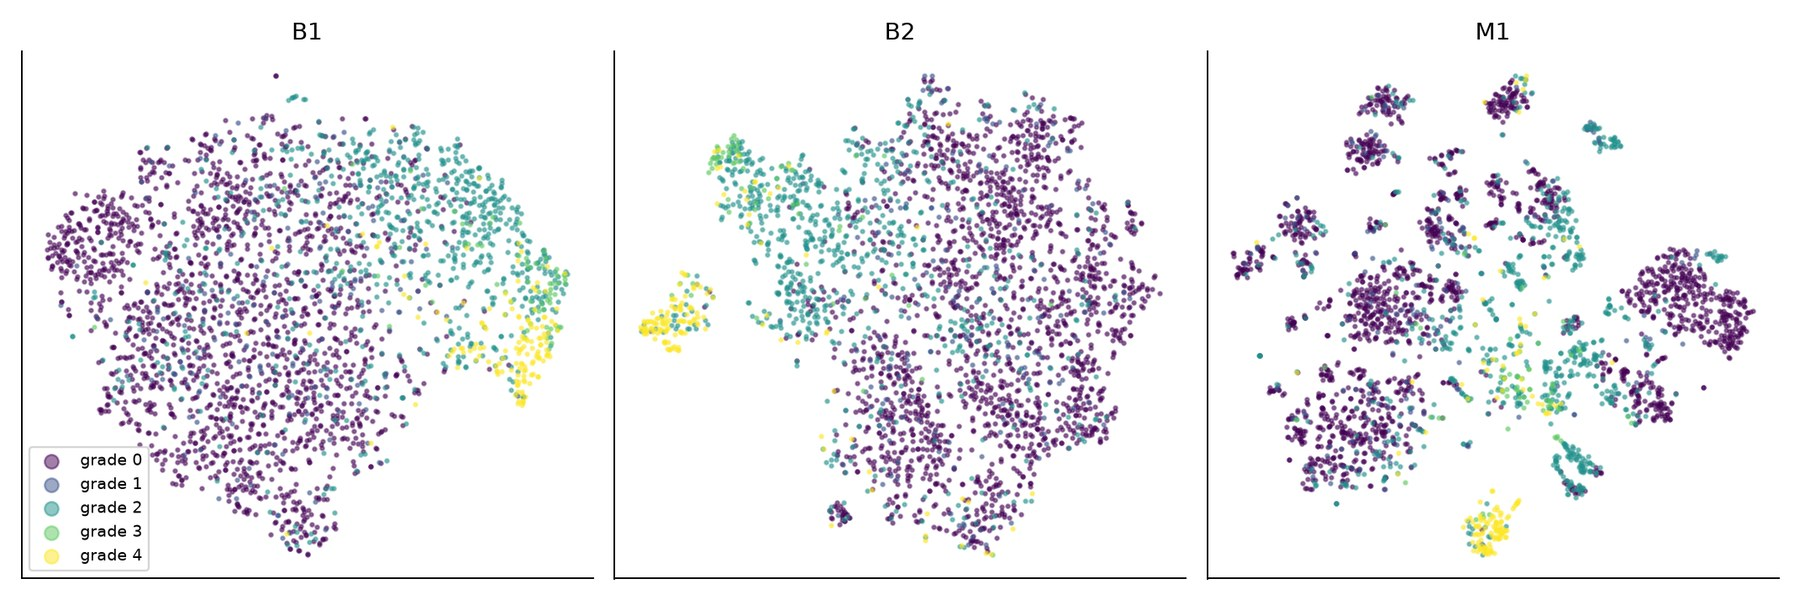
\includegraphics[width=0.9\textwidth]{figures/a04_tsne_grade.jpg}
    \caption{The same t-SNE embeddings coloured by DR grade.}
    \label{fig:tsne_grade}
\end{figure}

For B1 and B2 the two datasets overlap over large parts of the embedding, although each tends to occupy its own side. For M1 they fall into almost completely separate clusters. A measure that does not depend on the two-dimensional projection confirms this: in the standardised feature space, the fraction of the five nearest neighbours that come from the other dataset is 0.22 for B1, 0.19 for B2 and only 0.03 for M1 (a value near 0.5 would mean perfect mixing). The expectation of Section~\ref{subsec:diagnostics}, that retina-specific pre-training makes the representation less dependent on the imaging domain, is therefore not met: the M1 features separate the two sources most clearly. This separation did not translate into a measurable loss of QWK for M1, so domain separability and grading performance are not the same thing. Coloured by grade (Figure~\ref{fig:tsne_grade}), every model gathers most grade-4 images in one region or island and places grades~2 and~3 next to each other, while grade~1 is scattered among grade~0, in line with its very low recall.

\subsection{Summary of the Hypotheses}
\label{subsec:hypotheses_summary}

Table~\ref{tab:hypotheses} compares the two hypotheses of Section~\ref{subsec:research_question} with the results.

\begin{table}[!htbp]
    \centering
    \caption{Outcome of the two hypotheses.}
    \label{tab:hypotheses}
    \small
    \begin{tabularx}{\textwidth}{>{\raggedright\arraybackslash}p{4cm} >{\raggedright\arraybackslash}X >{\raggedright\arraybackslash}p{3cm}}
        \toprule
        \textbf{Hypothesis} & \textbf{Evidence} & \textbf{Outcome} \\
        \midrule
        H1: M1 $>$ B2 on DDR (QWK) & M1 0.682, B2 0.713; M1~$-$~B2 $=-0.031$ [$-0.051$, $-0.009$]; ordinal decoding: 0.707 vs 0.734 & Not supported; B2 scored higher \\
        H2: smaller in-to-out drop for M1 than for B1 & $\Delta$QWK M1 $-0.012$, B1 $0.003$; difference $-0.012$ [$-0.037$, $0.013$]; prior-matched $-0.008$ [$-0.041$, $0.023$] & Not distinguishable \\
        \bottomrule
    \end{tabularx}
\end{table}

In this experiment, retina-specific pre-training did not give the expected advantage: M1 was behind the ImageNet-pre-trained ViT-L on DDR and not measurably different from the much smaller ResNet-50, and none of the three models lost a measurable amount of QWK from EyePACS to DDR. These statements hold for this recipe, this input size, this one source--target pair and a single seed per ViT-L model. They are not evidence that RETFound is a weaker encoder in general; the official recipe differs from ours in training length and augmentation. Chapter~\ref{chap:projected_impact} discusses what follows from this.

\section{User Interface}
\label{sec:user_interface}

The demo application described in Section~\ref{subsec:demo_design} was implemented with Gradio and runs on the CPU of a laptop without a GPU. It loads the B2 checkpoint (ViT-L with ImageNet MAE pre-training), the model with the highest EyePACS-validation QWK (Section~\ref{subsec:training_dynamics}); the choice of the demo model therefore does not use any test result. The code is in the \texttt{code/demo} folder of the project repository. The interface is in English and intentionally simple: one page with an upload area, one button and the result panels.

\subsection{Upload Page}
\label{subsec:ui_upload}

Figure~\ref{fig:demo_upload} shows the page when it is opened. The title and the first line state which model is used. The note ``Research prototype of the SIC capstone project -- not a medical device'' is always visible, because the model was trained on a public research dataset and has not been validated clinically. The user drags a colour fundus photograph into the image box (or uses the upload button, the webcam or the clipboard) and presses \emph{Grade image}.

\begin{figure}[htbp]
    \centering
    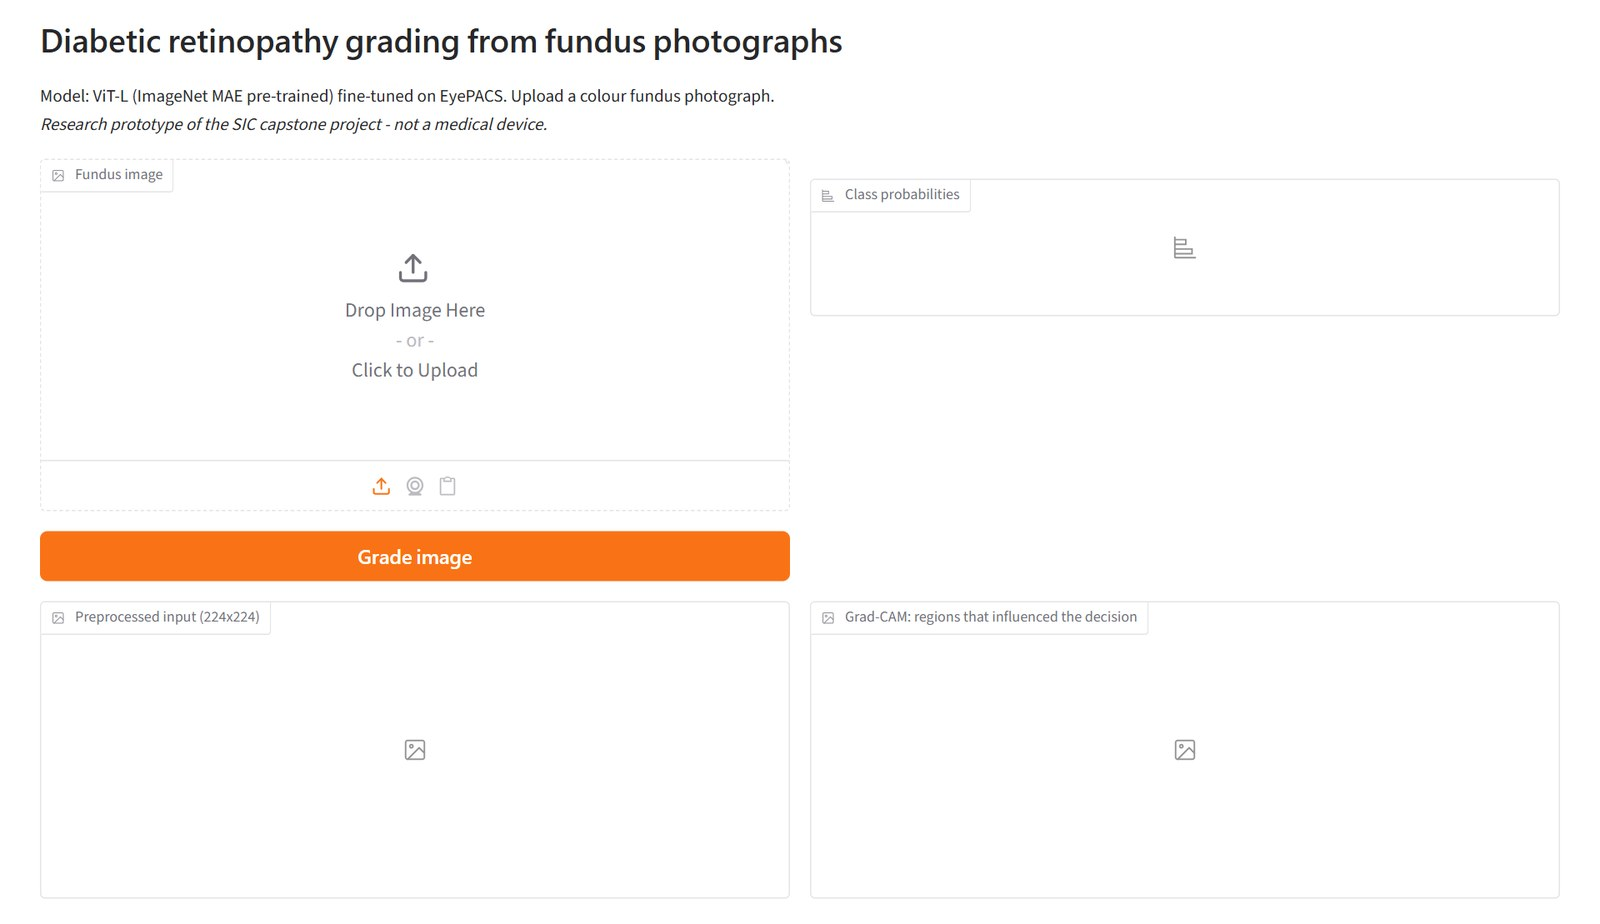
\includegraphics[width=0.85\textwidth]{figures/u01_demo_upload.jpg}
    \caption{Demo application before an image is uploaded: image input on the left, result panels (empty) on the right.}
    \label{fig:demo_upload}
\end{figure}

\subsection{Prediction Page}
\label{subsec:ui_result}

Figure~\ref{fig:demo_result} shows the result for a DDR-test image of reference grade~3 (severe NPDR). The application crops and resizes the photograph as in training and displays this $224\times224$ input, so that the user can check what the model actually received. It then shows (i) the predicted grade (here ``3 -- Severe'', which agrees with the reference), (ii) the probability of every grade as a bar chart (89\% for grade~3, 6\% for grade~4, 3\% for grade~2, 2\% for grade~1, 1\% for grade~0), (iii) the summed probability of referable DR, grade $\geq 2$ (97.1\%), with the recommendation ``refer to an ophthalmologist'' when it is at least 50\%, and (iv) a Grad-CAM overlay in which the colour from blue to red marks how strongly each image region influenced the decision. This single example illustrates the interface and says nothing about the accuracy of the model, which is reported in Section~\ref{sec:modeling}.

\begin{figure}[htbp]
    \centering
    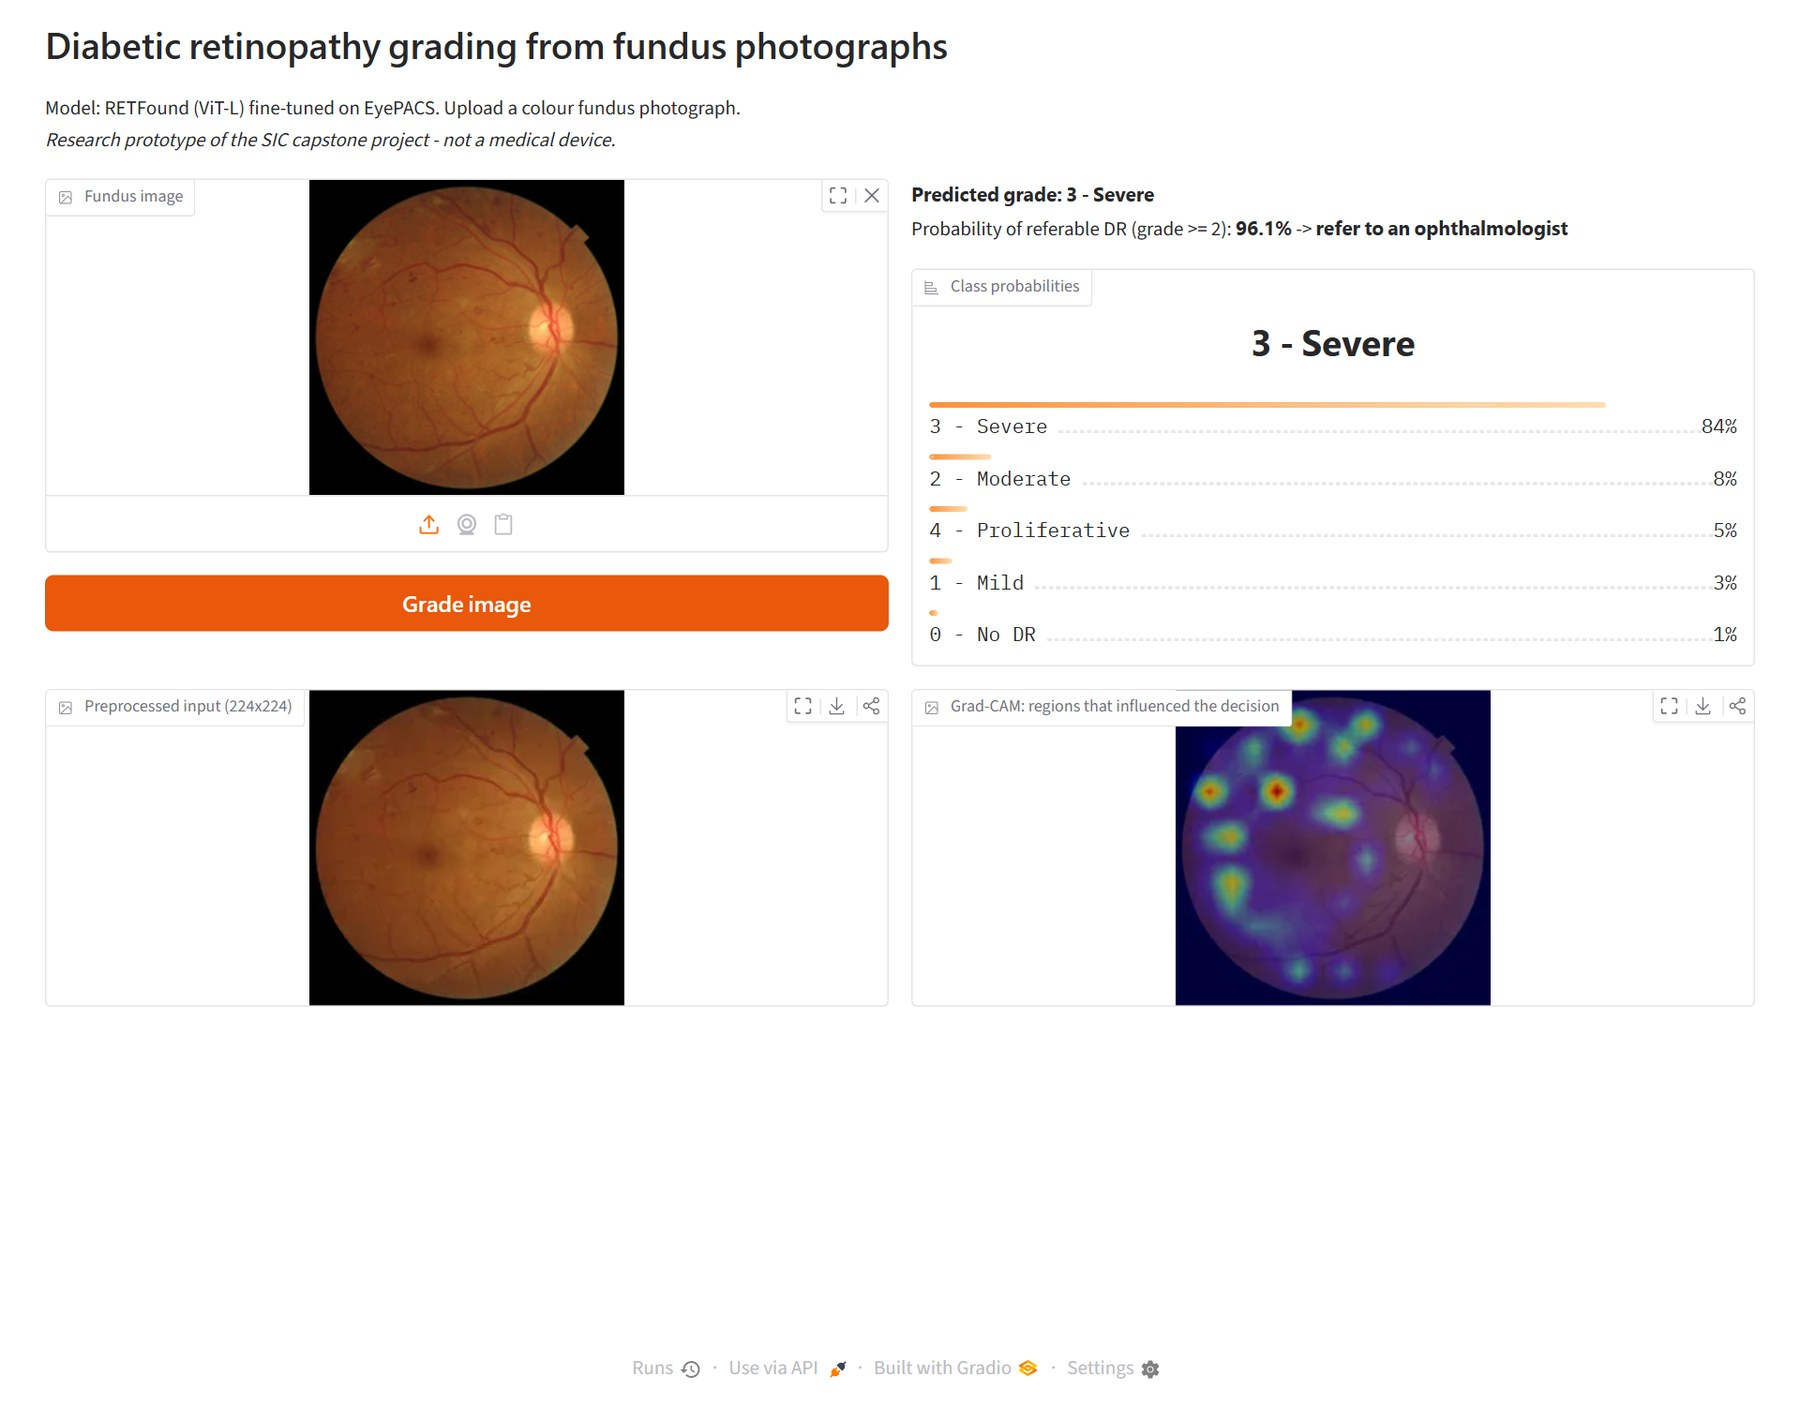
\includegraphics[width=0.85\textwidth]{figures/u02_demo_result.jpg}
    \caption{Demo application after grading a DDR-test image: predicted grade and referral hint (top right), class probabilities, the preprocessed input (bottom left) and the Grad-CAM overlay (bottom right).}
    \label{fig:demo_result}
\end{figure}

Showing the probabilities and the referable-DR probability, instead of a single label, lets the user see when the model is uncertain, which is important for a screening aid. The Grad-CAM panel is a plausibility check, not a lesion detector (Section~\ref{subsec:interpretability}). On a laptop CPU the grading of one image, including the Grad-CAM computation, takes a few seconds.

\section{Testing and Improvements}
\label{sec:testing_improvements}

\subsection{Software and Pipeline Tests}
\label{subsec:sw_tests}

Because every GPU hour is scarce, the code was tested on the local CPU with synthetic data before it was sent to Kaggle. The training library was run end to end with a very small Vision Transformer on 60 generated images: data loading, the square-root sampler, the cosine schedule, validation, checkpointing, the final evaluation of the two test sets and the saving of logits and features all worked. The pre-trained weights of B1, B2 and M1 were loaded on the CPU, and the lists of missing and unexpected keys were checked: only the classification head and the final normalisation layer were newly initialised, as intended. The prediction function used in the final evaluation was compared with the ordinary forward pass of the network, for ResNet-50 and for a ViT, and the logits were identical. The analysis script (metrics, bootstrap, figures, t-SNE and the generated LaTeX tables) was tested on synthetic predictions with known structure; the same test exposed one error in our own test data, which had different labels for different models, and led us to add an automatic check that all runs of a test set use the same label order. A short benchmark on the real Kaggle GPUs (about 2.7 minutes) verified that the three model types train, validate and save correctly, and measured speed and memory (Section~\ref{subsec:finetune}).

\subsection{Data Validation Tests}
\label{subsec:data_tests}

The label files were checked against the published sizes, patient identifiers were checked for leakage across splits, every cached image was checked for existence and size, and the EyePACS--DDR duplicate check described in Section~\ref{subsec:prep_dup} was validated with a self-test in which artificially degraded copies of DDR images had to be found again.

\subsection{Problems Found and Improvements Made}
\label{subsec:improvements}

\begin{itemize}[leftmargin=1.5em]
    \item \textbf{Duplicate check.} The first version, a 64-bit hash, flagged 94\% of the DDR images as ``near-duplicates''. It was replaced by a correlation test of a vessel-sensitive descriptor with a self-test (Section~\ref{subsec:prep_dup}); the new test found no duplicate.
    \item \textbf{Slow packaging of 92{,}000 small files.} Downloading the cache file by file hit the rate limit of the Kaggle interface, so the cache was repacked into four archive files; this also made the test sets separable from the training data.
    \item \textbf{Report build.} The first compile on the free Overleaf plan exceeded its time limit; the figures were compressed, two layout warnings were fixed, and the report is now built locally with MiKTeX.
    \item \textbf{Longer training.} A first set of 5-epoch pilot runs reached a QWK of only about 0.7, and the team assumed that the models were under-trained. A continuation attempt and an 8-epoch attempt were started; the 8-epoch session was cancelled by the platform because the session timeout had been set to 150 minutes instead of the full run length. All pilot results were discarded and all models were retrained from scratch for 15 epochs with a session timeout of 12 hours. The longer runs did not confirm the assumption: the best validation QWK stayed near 0.70 (Section~\ref{subsec:training_dynamics}), so the number of epochs was not the main limit.
    \item \textbf{GPU scheduling.} Kaggle allows only one of our two-GPU sessions at a time, so the runs are executed in sequence, with one model per GPU inside each session.
\end{itemize}

\subsection{Error Analysis}
\label{subsec:error_analysis}

Table~\ref{tab:errors} summarises the arg-max errors on DDR-test (3{,}759 images; seed-0 runs).

\begin{table}[htbp]
    \centering
    \caption{Structure of the arg-max errors on DDR-test (seed-0 runs). ``Grade 2 as 0'' is the share of the 1{,}344 grade-2 images that are predicted as no DR; referable sensitivity and specificity use predicted grade $\geq 2$.}
    \label{tab:errors}
    \small
    \begin{tabularx}{\textwidth}{X c c c}
        \toprule
        \textbf{Quantity} & \textbf{B1} & \textbf{B2} & \textbf{M1} \\
        \midrule
        Wrong images (\% of all)            & 32.4 & 31.8 & 40.4 \\
        Within one grade (\% of all)        & 80.9 & 84.0 & 81.6 \\
        Errors of exactly one grade (\% of errors) & 40.9 & 49.7 & 54.3 \\
        Errors of two or more grades (\% of errors) & 59.1 & 50.3 & 45.7 \\
        Under-grading (\% of errors)        & 62.9 & 58.5 & 49.1 \\
        Grade 2 as 0 (\% of grade 2)        & 32.7 & 29.9 & 33.0 \\
        Referable sensitivity (\%)          & 67.3 & 71.0 & 67.4 \\
        Referable specificity (\%)          & 93.1 & 94.4 & 91.3 \\
        \bottomrule
    \end{tabularx}
\end{table}

Between 46\% and 59\% of the errors miss by two grades or more, and the largest single source is moderate disease (grade~2) predicted as no DR, which happens for roughly one grade-2 image in three with every model. Grade~1 is rarely recognised: most of its 189 images are predicted as grade~0. These two error types are clinically relevant, because with the arg-max rule 29--33\% of the referable eyes (grade $\geq 2$) would not be referred by the seed-0 models. A plausible reason is that microaneurysms and small haemorrhages cover only a few pixels at $224\times224$, but this was not tested by an experiment. Among the seed-0 runs, M1 makes the most errors and over-grades more often than B1 and B2: many grade-0 and grade-2 images are moved to a higher grade. The second seed of B1 has 40.5\% wrong images, as many as M1, so a difference of this size can also arise from a change of seed alone. Examples of correct and wrong cases are shown with their Grad-CAM maps in Figure~\ref{fig:gradcam}.

\subsection{Limitations}
\label{subsec:limitations}

The following limitations apply to all conclusions of this report.
\begin{itemize}[leftmargin=1.5em]
    \item Only one source domain (EyePACS) and one target domain (DDR) were used, so the findings concern the transfer EyePACS $\rightarrow$ DDR and should not be generalised to other hospitals or cameras.
    \item RETFound's pre-training included about 9.8\% EyePACS images (without labels), so the in-domain EyePACS-test score of M1 may be optimistic; DDR was not part of the pre-training.
    \item DDR grade~3 has only 71 test images, so its recall and F1 have wide confidence intervals.
    \item No domain-generalization method (augmentation or domain-invariant learning) was applied; a model with domain-shift augmentation (M2) was planned but dropped because the GPU quota allowed only two ViT-L runs in parallel. The study therefore measures the robustness of pre-trained representations only.
    \item \textbf{Training budget.} All models were trained for 15 epochs, the largest number that fitted the free GPU quota; the official RETFound recipe uses more. The validation QWK had flattened before epoch~15 (Figure~\ref{fig:curves}), but this does not show that a different recipe or a longer schedule would also stop at the same level.
    \item B2 and M1 were trained with a single seed and B1 with two; the bootstrap intervals measure the sampling noise of the test images, not the variation between training runs, so small differences between M1 and B2 should not be over-interpreted.
    \item All images were reduced to $224\times224$ pixels, which hides small lesions and probably limits the recognition of grade~1; the absolute QWK is therefore below the values published for high-resolution systems, and the conclusions concern the \emph{relative} behaviour of the models under identical conditions.
    \item EyePACS labels come from a single grader per image and are noisy, whereas DDR was graded by a team of seven trained graders (Section~\ref{subsec:ddr}); part of any difference between the two test sets may come from this difference in label quality.
\end{itemize}


\chapter{Projected Impact}
\label{chap:projected_impact}

\section{Accomplishments and Benefits}
\label{sec:accomplishments}

\subsection{What Was Achieved}
\label{subsec:achieved}

The project delivered a complete, reproducible experiment on the robustness of diabetic retinopathy grading across fundus datasets:
\begin{itemize}[leftmargin=1.5em]
    \item a preprocessing pipeline that converted about 92{,}000 EyePACS and DDR photographs into a common $224\times224$ format, with quality checks, a verified absence of duplicates between the two datasets, and a strict separation of data roles in which DDR is used only once, for the final test;
    \item a training library with the RETFound fine-tuning recipe (layer-wise learning-rate decay, label smoothing, square-root balanced sampling, mixed precision) that runs the comparison on free Kaggle T4 GPUs, with one independent job per GPU;
    \item a controlled comparison of three models (B1 ResNet-50, B2 ViT-L with ImageNet MAE weights, M1 RETFound) with QWK as the primary metric, bootstrap confidence intervals, a prior-matched in-domain versus out-of-domain comparison and an ordinal-decoding variant;
    \item diagnostic analyses (confusion matrices, per-grade recall, ROC for referable DR, error structure, Grad-CAM and t-SNE) and a working English web demo that grades an uploaded fundus photograph and shows the probabilities and a Grad-CAM overlay.
\end{itemize}

\subsection{Main Findings}
\label{subsec:main_findings}

% [PENDING: written after the final results: QWK on DDR and EyePACS for M1, B2, B1; whether H1 and H2 are supported; the effect of the decision rule; what Grad-CAM and t-SNE show]

\subsection{Benefits}
\label{subsec:benefits}

\begin{itemize}[leftmargin=1.5em]
    \item \textbf{For screening practice.} An automated assistant trained on one public dataset and evaluated on a dataset collected in another country shows how far such a tool can support primary-care screening where ophthalmologists are scarce. The demo shows how a tool could present its result with probabilities and a visual explanation.
    \item \textbf{For model selection.} The study gives practitioners a concrete warning: a better in-domain score or a larger pre-training set does not guarantee a better score on a new device or population, and every deployment needs a local test set.
    \item \textbf{For students and future teams.} The scripts, logs and figures form a reproducible template for dataset-shift studies under a small compute budget (free GPUs only), including a leakage-controlled data protocol and a bootstrap-based way to judge differences.
\end{itemize}

\section{Future Improvements}
\label{sec:future_improvements}

\subsection{Limitations of This Study}
\label{subsec:limits_summary}

The limitations in Section~\ref{subsec:limitations} bound the conclusions: only one source and one target dataset, a single training seed for the ViT-L models, a training budget of 15 epochs, an input resolution of 224 pixels, and no domain-generalization method. The interval widths in this report measure only the sampling noise of the test set.

\subsection{Roadmap}
\label{subsec:roadmap}

\begin{enumerate}[leftmargin=1.5em]
    \item \textbf{Higher resolution.} Training at 448 or 512 pixels, with the position embeddings interpolated, should improve the recognition of mild disease (grade~1); this needs more GPU memory and time than the free quota allowed.
    \item \textbf{More seeds and longer schedules.} Three or more seeds per ViT-L model and 30--50 epochs would turn the single-run comparisons into statistically solid ones.
    \item \textbf{Domain-shift augmentation.} A fourth model, RETFound with augmentation that imitates camera differences (colour casts, gamma, blur, compression, as in GDRNet), was planned but could not be trained within the quota; it would show whether augmentation adds robustness on top of retinal pre-training.
    \item \textbf{More domains.} Adding more source datasets (for example Messidor-2 or APTOS) and more target datasets would show whether the findings hold beyond EyePACS $\rightarrow$ DDR and enable leave-one-domain-out evaluation.
    \item \textbf{Methods that target the domain gap directly.} Examples are test-time adaptation of the normalisation statistics, continued self-supervised pre-training on unlabelled target-domain photographs, and training objectives that encourage domain-invariant features.
    \item \textbf{Ordinal and calibrated outputs.} Training with an ordinal loss and calibrating the probabilities would use the grade order during training, not only at decoding, and would make the referral recommendation of the demo more reliable.
    \item \textbf{Clinical validation.} Any real use requires prospective validation with ophthalmologists, a study of fairness across devices and populations, and regulatory review; the present demo is a research prototype only.
\end{enumerate}

\chapter{Team Member Review and Comment}
\label{chap:team_review}

% ------------------------------------------------------------------------------
% TEAM PICTURE SECTION
% ------------------------------------------------------------------------------
\begin{figure}[htbp]
    \centering
    \includegraphics[height=7cm]{figures/team_member_1.jpg}\hspace{0.8cm}%
    \includegraphics[height=7cm]{figures/team_member_2.jpg}
    \caption{Capstone Project Team Photograph (the two members of \teamName)}
    \label{fig:team_photo}
\end{figure}

\vspace{0.3cm}

% ------------------------------------------------------------------------------
% TEAM MEMBERS REVIEW AND COMMENT TABLE
% Matches exact structure and palette of the source document (#DEE5FA fill, #BFBFBF borders)
% ------------------------------------------------------------------------------
\noindent
\begin{table}[htbp]
    \centering
    \caption{Individual Team Member Reviews and Comments}
    \label{tab:team_member_comments}
    \renewcommand{\arraystretch}{1.35}
    \arrayrulecolor{SamsungGray}
    \begin{tabularx}{\textwidth}{|>{\raggedright\arraybackslash\sffamily}p{3.2cm}|>{\raggedright\arraybackslash}X|}
        \hline
        \rowcolor{SamsungLightBlue}
        \multicolumn{1}{|c|}{\sffamily\bfseries\color{SamsungDarkGray}NAME} & 
        \multicolumn{1}{c|}{\sffamily\bfseries\color{SamsungDarkGray}REVIEW and COMMENT} \\
        \hline
        \textbf{\memberOne} & \textbf{Role:} Model design and training.\newline
        \textbf{Tasks:} Baselines B1 and B2, RETFound fine-tuning (M1 and M2), training scripts and GPU-budget planning on Kaggle, Grad-CAM and t-SNE analysis, report writing and review.\newline
        \textbf{Self-review:}\newline\mbox{}\newline
        \textbf{Peer comment:}\newline\mbox{} \\
        \hline
        \textbf{\memberTwo} & \textbf{Role:} Data and evaluation.\newline
        \textbf{Tasks:} Dataset acquisition and verification, preprocessing, exploratory data analysis, metrics and bootstrap confidence intervals, testing, the Gradio web demo, report writing and review.\newline
        \textbf{Self-review:}\newline\mbox{}\newline
        \textbf{Peer comment:}\newline\mbox{} \\
        \hline
    \end{tabularx}
\end{table}

\chapter{Instructor Review and Comment}
\label{chap:instructor_review}

% ------------------------------------------------------------------------------
% INSTRUCTOR EVALUATION MATRIX
% Matches exact criteria, score weights, and styling of source document
% ------------------------------------------------------------------------------
\noindent
\begin{table}[htbp]
    \centering
    \caption{Capstone Project Evaluation Rubric and Instructor Feedback}
    \label{tab:instructor_evaluation}
    \renewcommand{\arraystretch}{2.0}
    \arrayrulecolor{SamsungGray}
    \begin{tabularx}{\textwidth}{|>{\raggedright\arraybackslash\sffamily\bfseries\color{SamsungBlue}}p{4.6cm}|>{\centering\arraybackslash\sffamily\bfseries}p{2.2cm}|>{\raggedright\arraybackslash}X|}
        \hline
        \rowcolor{SamsungLightBlue}
        \multicolumn{1}{|c|}{\sffamily\bfseries\color{SamsungDarkGray}CATEGORY} & 
        \multicolumn{1}{c|}{\sffamily\bfseries\color{SamsungDarkGray}SCORE} & 
        \multicolumn{1}{c|}{\sffamily\bfseries\color{SamsungDarkGray}REVIEW and COMMENT} \\
        \hline
        IDEA & \_\_/10 & \vspace{0.5cm} \\
        \hline
        APPLICATION & \_\_/30 & \vspace{0.5cm} \\
        \hline
        RESULT & \_\_/30 & \vspace{0.5cm} \\
        \hline
        PROJECT MANAGEMENT & \_\_/10 & \vspace{0.5cm} \\
        \hline
        PRESENTATION \& REPORT & \_\_/20 & \vspace{0.5cm} \\
        \hline
        \rowcolor{SamsungLightBlue!40}
        TOTAL & \_\_/100 & \vspace{0.5cm} \\
        \hline
    \end{tabularx}
\end{table}

\vspace{0.8cm}

\noindent
\begin{minipage}{\textwidth}
    \raggedleft
    \sffamily
    \textbf{Instructor Signature:}\hspace{4.5cm}\textbf{Date:}\hspace{2.5cm}\par
    \vspace{1.5cm}
    \textbf{\instructorName}\hspace{6.5cm}
\end{minipage}


% ------------------------------------------------------------------------------
% 4. BIBLIOGRAPHY (IEEE Reference Style via BibLaTeX/Biber)
% ------------------------------------------------------------------------------
\clearpage
\nocite{*} % Show example entries in references.bib
\printbibliography[heading=bibintoc,title={References}]

% ------------------------------------------------------------------------------
% 5. APPENDICES
% ------------------------------------------------------------------------------
\clearpage
\appendix
\chapter{Source Code and Implementation Details}
\label{app:code}

This appendix provides key excerpts of the core model pipeline implementation.

\begin{lstlisting}[language=Python, caption={Core Training Loop and Metric Evaluation Pipeline}, label={lst:training_loop}]
import torch
import torch.nn as nn
from torch.utils.data import DataLoader

def train_one_epoch(model: nn.Module, 
                    dataloader: DataLoader, 
                    optimizer: torch.optim.Optimizer, 
                    criterion: nn.Module, 
                    device: torch.device) -> float:
    """
    Executes a single epoch pass over the training dataset.
    """
    model.train()
    running_loss = 0.0
    for batch_idx, (inputs, targets) in enumerate(dataloader):
        inputs, targets = inputs.to(device), targets.to(device)
        
        optimizer.zero_grad()
        outputs = model(inputs)
        loss = criterion(outputs, targets)
        loss.backward()
        optimizer.step()
        
        running_loss += loss.item() * inputs.size(0)
        
    epoch_loss = running_loss / len(dataloader.dataset)
    return epoch_loss
\end{lstlisting}

\chapter{Hyperparameter Configurations}
\label{app:hyperparameters}

\begin{table}[htbp]
    \centering
    \caption{Detailed Experimental Hyperparameter Settings}
    \label{tab:hyperparameters}
    \begin{tabularx}{\textwidth}{l l X}
        \toprule
        \textbf{Hyperparameter} & \textbf{Selected Value} & \textbf{Description / Search Space} \\
        \midrule
        Base Learning Rate      & $1 \times 10^{-4}$      & Cosine Annealing scheduler with warm restart \\
        Batch Size              & 32                      & Optimized for GPU memory throughput \\
        Optimizer               & AdamW                   & $\beta_1 = 0.9, \beta_2 = 0.999, \text{weight\_decay} = 0.01$ \\
        Training Epochs         & 100                     & Early stopping with patience of 10 epochs \\
        Input Resolution        & $224 \times 224$        & Standard input tensor dimensions \\
        Loss Function           & Cross-Entropy           & Label smoothing $\alpha = 0.1$ \\
        \bottomrule
    \end{tabularx}
\end{table}


\end{document}
